%%% Exemplo de utilizao da classe ITA
%%%
%%%   por        Fbio Fagundes Silveira   -  ffs [at] ita [dot] br
%%%              Benedito C. O. Maciel     -  bcmaciel [at] ita [dot] br
%%%              Giovani Volnei Meinertz   -  giovani [at] ita [dot] br
%%%
%%%  IMPORTANTE: O texto contido neste exemplo nao significa absolutamente nada.  :-)
%%%              O intuito aqui eh demonstrar os comandos criados na classe e suas
%%%              respectivas utilizacoes.
%%%
%%%  $Id: ExemploTeseITA.tex 17 2006-02-07 17:59:17Z ffs $
%%%  $HeadURL: file:///opt/repositorioITALUS/classeITA/tags/versao-2.1/ExemploTeseITA.tex $
%%%
%%% ITALUS
%%% Technological Institute of Aeronautics --- ITA
%%% Sao Jose dos Campos, Brazil
%%% HomePages:        http://www.comp.ita.br/italus
%%%                   http://groups.yahoo.com/group/italus/
%%% Discussion list: italus {at} yahoogroups.com
%%%
%++++++++++++++++++++++++++++++++++++++++++++++++++++++++++++++++++++++++++++++
% Parametros da classe ITA:
%   msc   = Tese de Mestrado    --> no ITA, Dissertacao eh Tese ...  :-)
%   dsc   = Tese de Doutorado
%   quali = Exame de Qualificacao
%   dv    = 'Draft Version'     --> imprime 'Versao Preliminar + data no rodape
%   fem   = Doutora
%   eng   = para teses em ingls
%++++++++++++++++++++++++++++++++++++++++++++++++++++++++++++++++++++++++++++++
\documentclass[msc,eng]{ita}    % ITA.cls based on standard book.cls
\usepackage{amssymb,amsmath}
\usepackage{graphicx}
\usepackage[latin1]{inputenc}
\usepackage{placeins}
\usepackage{subfig}
\bibliographystyle{abnt-alf-eng}
%++++++++++++++++++++++++++++++++++++++++++++++++++++++++++++++++++++++++++++++
% Identificacoes...
%++++++++++++++++++++++++++++++++++++++++++++++++++++++++++++++++++++++++++++++
\course{Aeronautics and Mechanical Engineering}
\dept{Energy Division}
\area{Aerodynamics, Propulsion and Energy.}

% Autor do trabalho: Nome Sobrenome
\author{Rodrigo Badia}{Piccinini}

% Endereco do Autor -> utilizado no verso da folha de rosto
% Obrigatorio para Teses
\itaauthoraddress{Rua Mal Andrea, 238, apto 401, Pituba.}{41810-105}{Salvador--BA}

% Titulo da Tese/Dissertacao
\title{Eulerian-Lagrangian simulation of a turbulent evaporating spray}

% Orientador
\advisor{Prof.~Dr.}{Marcelo J.S. de Lemos}

% Co-orientador opcional
% \coadvisor{Prof.~Dr.}{Beltrano de Tal}{OVNI}

% Chefe da divisao de Pos-Graduacao
% Obrigatrio para Teses
\boss{Prof.~Dr.}{Celso Massaki Hirata}

% Banca Examinadora
% Obrigatrio para Teses
\examiner{Prof. Dr.}{Cl\'{a}udia Regina de Andrade}{Chairperson}{ITA}%
\examiner{Prof. Dr.}{Fernando de Souza Costa}{}{INPE}%
\examiner{Prof. Dr.}{\'{E}zio C. Garcia}{}{ITA}%
%\examiner{Prof. Dr.}{Quarto}{Membro}{ITA}%

% Data da defesa
\date{}{2011}

% Palavras-Chaves informadas pela Biblioteca -> utilizada na CIP
% Obrigatrio para Teses

\kwcip{Pulverizadores; Escoamento multif\'{a}sico}
\kwcip{Combust\~{a}o}
\kwcip{M\'{e}todo de volumes finitos}
\kwcip{An\'{a}lise num\'{e}rica}
\kwcip{Simula\c{c}\~{a}o do escoamento}
\kwcip{F\'{i}sica}
%\kwcip{xxx}

% Glossario
\makeglossary
\frontmatter

\begin{document}

%Definitions
\newcommand{\bv}[1]{\mathbf{#1}} 
\newcommand{\req}[1]{#1^{*}} 

%environments
\newenvironment{remark}[1][Remark.]{\begin{trivlist}
\item[\hskip \labelsep {\bfseries #1}]}{\end{trivlist}}

\newenvironment{notation}[1][Notation.]{\begin{trivlist}
\item[\hskip \labelsep {\bfseries #1}]}{\end{trivlist}}

% Folha de Rosto
\maketitle

% Dedicatoria
\begin{itadedication}
\`{A} Dora Badia, aos meus pais e aos meus irm\~{a}os.
\end{itadedication}

% Agradecimentos
\begin{itathanks}
Eu agrede�o � minha fam�lia pelo apoio e pelas oportunidades que tive.

Agrade�o ao Prof. Marcelo J.S. de Lemos pela orienta��o e pela ajuda com os recursos computacionais. Para mim, foi um privil�gio trabalhar sob orienta��o de um pesquisador de sucesso exemplar.

Agrade�o � Sygma Motors, nominalmente a Marcos Langeani, onde iniciei minha vida profissional e a quem sou grato pelas oportunidades e pelo aprendizado oferecidos.

Agrade�o ao Prof. Francisco Jos� de Souza pelo aprendizado, pelo incentivo ao estudo da mec�nica dos fluidos e pelo exemplo profissional.

Agrade�o aos ex-colegas Carla Fernandes, Clayton Zabeu, Edilson Viana, Felipe Tannus Dorea, Gustavo Hindi, Jos� Eduardo de Oliveira, Marcelo Andreotti e Oswaldo Fran�a Jr pelo companheirismo e pelo aprendizado.

Agrade�o ao Prof. Fl�vio Luiz Cardoso Ribeiro, procurador para os tr�mites burocr�ticos do ITA, colega no curso de gradua��o em engenharia aeron�utica e um dos meus melhores amigos, pelo apoio � conclus�o dos estudos do mestrado.

Agrade�o � Blandina Oliveira pela ajuda com a impress�o e com a distribui��o das c�pias da disserta��o.

Agrade�o �s comunidades de c�digo aberto que mant�m softwares de qualidade disponibilizados sem custo pelo simples esp�rito de colabora��o.

Este trabalho come�ou na quase sub-tropical S�o Jos� dos Campos e foi finalizado em Salvador, no cora��o do Brasil.

\end{itathanks}
% 
% Epgrafe
\thispagestyle{empty}
\ifhyperref\pdfbookmark[0]{\nameepigraphe}{epigrafe}\fi
\begin{flushright}
\begin{spacing}{1}
\mbox{}\vfill
{\sffamily\itshape
We see only what we know.
\\}
--- \textsc{Johann Wolfgang von Goethe}
\end{spacing}
\end{flushright}

% Resumo
\begin{abstract}

Este trabalho consistiu na simula��o num�rica de um spray: um escoamento bif�sico composto por uma fase gasosa e uma fase l�quida. A fase gasosa � tratada como um meio cont�nuo, e a fase l�quida � tratada com um conjunto de gotas dispersas na fase gasosa. Foi aplicada a aproxima��o assint�tica de baixo n�mero de Mach para a fase gasosa com o objetivo de modelar varia��es da densidade causadas por gradientes de temperatura sem o envolvimento de complica��es existentes na formula��o de um escoamento compress�vel. Os efeitos da turbul�ncia na fase gasosa foram modelados utilizando o conceito de viscosidade turbulenta governada por duas equa��es diferenciais que comp�e o assim denominado modelo \textit{k-epsilon}. A fase l�quida dispersa foi modelada como part�culas-pontos, �s quais s�o atribu�das propriedades termodin�micas e modelos 0-d para c�lculos de transfer�ncia de momento, energia e massa. A fase gasosa foi discretizada segundo o m�todo de volumes finitos. Os resultados num�ricos foram comparados com medi��es experimentais e indicaram que a metodologia utilizada descreve razoavelmente bem o spray. Foram verificadas, por�m, subestimativas da velocidade e da taxa de evapora��o das gotas com rela��o �s medi��es experimentais.

\end{abstract}
% Palavras Chave
% No manual nao consta palavras-chaves
%\keywords{Teses, Estilos, Italus}

% Abstract
\begin{englishabstract}

This work consists in a numerical simulation of a spray jet: a two-phase flow composed by a gaseous and a liquid phase. The gaseous phase is treated as a continuous medium, and the liquid phase is treated as a dispersed phase. An asymptotic approximation of zero Mach number was applied to the gaseous phase in order to account for density variations due to temperature gradients without dealing with extra complexities of the fully compressible flow formulation. The effects of turbulence on the gas flow were modeled using the concept of turbulent viscosity determined by a system of two partial differential equations, the so called k-epsilon model. The liquid dispersed phase was modeled as point-particles, to whom thermodynamic properties and 0-d models for momentum, heat and mass transfers were assigned. The gaseous phase was discretized and numerically solved using the finite volume method. The numerical results were compared to measurements and a reasonable prediction was found. It was verified, though, underestimations of droplet velocity and evaporation rate.

\end{englishabstract}
% Keywords
% Idem Palavras-chaves ...
%\englishkeywords{Theses, Styles, Italus}

% sumario
\tableofcontents
% lista de figuras
\listoffigures
% lista de tabelas
\listoftables
% lista de abreviaturas
%\listofabbreviations
% \input{abreviaturas}
% lista de simbolos
\listofsymbols
%\section{Latin Characters:}

\begin{longtable}{ll}
\textbf{Latin Characters:} & \\
$C_D$ & doplet drag coefficient \\
$c_p$ & specific heat at constant pressure [$J/kg/K$] \\
$c_v$ & specific heat at constant volume [$J/kg/K$]\\
$D$ & droplet diameter [$m$]\\
$\tilde{f}$ & favre-average of function $f$\\
$f''$ & deviation of favre-averaged function $\tilde{f}$\\
$\bar{f}$ & time-average of function $f$\\
$f'$ & deviation of time-averaged function $\bar{f}$\\
$\bv{g}$ & vector field of gravity force [$m/s^2$]\\
$\dot{m}_d$ & injection liquid mass rate [$kg/s$]\\
$\dot{m}_{g}$ & gas mass rate [$kg/s$]\\
$\dot{m}_{ac}$ & acetone vapor mass rate [$kg/s$]\\
$h_d$ & droplet enthalpy [$J/kg$]\\
$h_s$ & gas sensible enthalpy [$J/kg$]\\
$h$ & gas enthalpy [$J/kg$]\\
$k$ & turbulent kinetic energy [$J/kg$]\\
$L_v$ & latent heat of vaporization [$J/kg$]\\
$m_d$ & droplet mass [$kg$]\\
$M$ & Mach number \\
$p_{\infty}$ & pressure at far-field boundary [$Pa$]\\
$p_{0}$ & thermodynamic pressure [$Pa$]\\
$p_{2}$ & dynamic pressure [$Pa$]\\
$p$ & pressure [$Pa$]\\
$Pr$ & gas Prandtl number \\
$Re$ & gas Reynolds number \\
$\bv{S}$ & strain tensor [$1/s$]\\
$S_{hs}$ & spray enthalpy source term [$J/m^3/s$]\\
$S_{m}$ & spray mass source term [$kg/m^3/s$]\\
$S_{mom}$ & spray momentum source term [$kg/m^3/s$]\\
$S_{Y_k}$ & spray source term of species k [$kg/m^3/s$]\\
$Sc$ & gas Schmidt number \\
$Sh$ & gas Sherwood number \\
$St$ & Stokes Number \\
$T_d$ & droplet temperature [$K$]\\
$T$ & gas temperature [$K$]\\
$t$ & time [$s$]\\
$\bv{U}$ & gas velocity vector [$m/s$]\\
$\bv{U}_d$ & droplet velocity vector [$m/s$]\\
$\bv{U}_{slip}$ & droplet velocity vector relative to the gas [$m/s$]\\
$\bv{V}_k$ & diffusion velocity of species k [$m/s$]\\
$x$ & axial coordinate [$m$]\\
$\bv{x}$ & position vector [$m$] \\
$y$ & radial coordinate [$m$]\\
$Y_k$ & mass fraction of species k\\
$W_k$ & molecular weight of species k [$kg/mol$]\\
\\

\textbf{Greek Characters:} & \\
$\alpha$ & thermal diffusivity [$m^2/s$]\\
$\gamma$ & ratio of constant pressure and constant volume specific heats \\
$\epsilon$ & dissipation rate of turbulent kinetic energy [$J/kg/s$]\\
$\kappa$ & thermal conductivity [$W/m/K$]\\
$\mu$ & gas dynamic viscosity [$Pa.s$]\\
$\rho$ & gas density [$kg/m^3$]\\
$\rho_d$ & droplet density [$kg/m^3$]\\
$\bv{\tau}$ & viscous stress tensor [$Pa$]\\
$\tau_e$ & droplet evaporation relaxation time [$s$]\\
$\tau_h$ & droplet heating relaxation time [$s$]\\
$\tau_u$ & droplet momentum relaxation time [$s$] \\
$\phi_{v,l}$ & liquid volume fraction \\
\\

\textbf{Special Characters:} & \\
cdf & cumulative density function\\
pdf & probability densitiy function\\
SMD & Sauter mean diameter \\
$\mathcal{D}_k$ & diffusion coefficient of species k [$m^2/s$]
\end{longtable}


\mainmatter
% Os capitulos comecam aqui

\chapter{Introduction}\label{chap: intro}
\section{Motivation}

The study of spray jets is important for several technical applications: gas turbines, furnaces, automotive and rocket engines.  An extensive presentation of spray applications may be found in \cite{liu2000science}, but any equipment or transportation powered by the combustion of a liquid fuel has its design, efficiency and environmental impact challenged by the proper description of processes such as: liquid atomization, droplet transport, inter-phase transfers and vapor mixing with oxygen. Notwithstanding the expected complexity of all said, spray jets are often turbulent. 

Studying the spray jet by means of computer modeling alongside with experimentation is still a growing activity in industry, specially in what concerns brazilian activities. One notable difficulty is the requirement of expensive computational and laboratorial resources as well as capable professionals to operate them, and there is always doubt about how predictive/descriptive computations/experiments may be.

Undoubtful are, though, the benefits that society might receive from the evolution of technical applications: fuel flexibility, lower emission levels, higher work efficiency, safer operability.

\section{Objective}
This thesis has the following objectives:
\begin{itemize}
  \item Implement a low Mach number formulation to allow modeling of gas density variations due to high temperature gradients while neglecting fluid compressibility.
  \item Review some existent models for droplet-gas heat, mass and momentum transfers under the framework of RANS\footnote{RANS: Reynolds-averaged Navier-Stokes equations.} modeling for gas turbulence;
  \item Compare computed quantities to measurements reported in the literature such as droplet velocity and diameter, vapor and liquid mass flux, gas velocity and turbulence properties.
\end{itemize}

\section{The Spray Jet and the Lagrangian Point-Particle Method}

A spray jet is a particular case of a dispersed multiphase flow originated by the instabilization of a liquid jet emerging in a gaseous atmosphere.  The spray is composed by a continuous gaseous phase and a dispersed phase of liquid droplets. 

Differently from many multiphase flows where the description of phase interfaces is of great importance, in the dispersed regime it is the volume fraction of each phase the determinant factor of their interaction. The liquid volume fraction in spray jets may span from low or dilute ($\phi_{v,l} < 10^{-3}$) to high or dense ($\phi_{v,l} > 10^{-3}$).

In dilute sprays, the dynamics of liquid droplets is mainly governed by the gas turbulence. Modeling such sprays may be concentrated on modeling the gas effect on droplets and neglecting the droplet effect on the gas (one-way coupling) or taking both ways into account (two-way coupling). For dense sprays, however, the interaction between droplets (collision and coalescence) become important and must also be modeled (four-way coupling). A review on the computational approaches for different volume fractions is given in \cite{balachandar2010turbulent}. 

This work deals with a dilute spray ($\phi_{v,l} \approx 2.1 \times 10^{-5}$). A two-way coupling modeling was used for averaged flow properties and a one-way coupling was used for turbulence modeling; that is, no direct influence of droplets is present in the turbulence model equations and they are identical to those for a pure gaseous flow.

In the modeling formulation used in this work, the droplets were treated as point-particles with assigned properties and instead of tracking an interface, the problem is to track the droplet position in the domain. The Lagrangian point-particle nomenclature comes from the fact that droplet motion is described by ordinary differential equations written in a Lagrangian reference frame. This, coupled with the gaseous phase being modeled by partial differential equations in an Eulerian refence frame is what is called the Eulerian-Lagrangian description of the spray.

The interaction droplet-gas is done by computing source/sink terms to the gaseous equations and the correct droplet position must be known to correctly distribute the spray source terms in the gas flow. The more droplets are represented in the domain, smoother are the computed source terms.

\section{Low Mach Number Approximation}

In a subsonic flow at low Mach number, pressure variations affect the continuity equation much more by changing the velocity field than by changing the fluid density. If heat transfer is present, though, temperature variations may cause considerable variations in fluid density; and continuity, momentum and energy equations must be solved in a coupled manner. Solving the equations in the original compressible formulation adds unwanted difficulties to the numerical solver and requires extra care with the boundary conditions to avoid wave interferences in the solution \cite{poinsot2005theoretical}.

One possible approach is the Boussinesq simplification, which neglects density variations everywhere except in the buoyancy term in the momentum equation. This decouples the energy equation from both the momentum and continuity equations, but it is limited to low temperature differences of about $15K$ \cite{ferziger}.

In the case of a spray jet, temperature variations may be much higher and mass source terms are present due to droplet evaporation. Neglecting local changes in density may thus cause significant errors in the solution.

A possible way to overcome the limitations of the Boussinesq approximation and the complexity of the fully compressible formulation is the asymptotic approximation of zero Mach number for the Navier-Stokes equations. The simplified equations have been formally derived in \cite{majda} and are further discussed in \cite{muller1999low} and \cite{viozat1997implicit}.

For the spray jet studied in this thesis, the maximum Mach number is found in the nozzle exit and it is less than $0.1$.

\section{Droplet Evaporation}

A comprehensive text on droplet evaporation and heating is presented in \cite{sirignano}, where some covered topics are the case of a single and spherically symmetric droplet in a quiescent gas, the effect of gas convection around the droplet, the extra complexities of a multi-component liquid droplet, droplet behavior near critical conditions and the heating and evaporation of a group of droplets nearly located.

As previously mentioned, this thesis deals with a dilute spray and thus droplets are considered to heat and vaporize similarly to a single and isolated droplet. The effects of gas convection are taken into account using empirically established laws. The liquid phase has one single component (acetone) and the droplets are far from critical conditions.

Some more simplifications are made regarding the radial transport of heat inside the droplet. They will be discussed as the heating and the evaporation models are presented, in Chapter \ref{chap: equations}.

\section{Turbulence and Droplet Submodels}

\begin{figure}[h]
 \centering
\begin{tabular}{cc}
 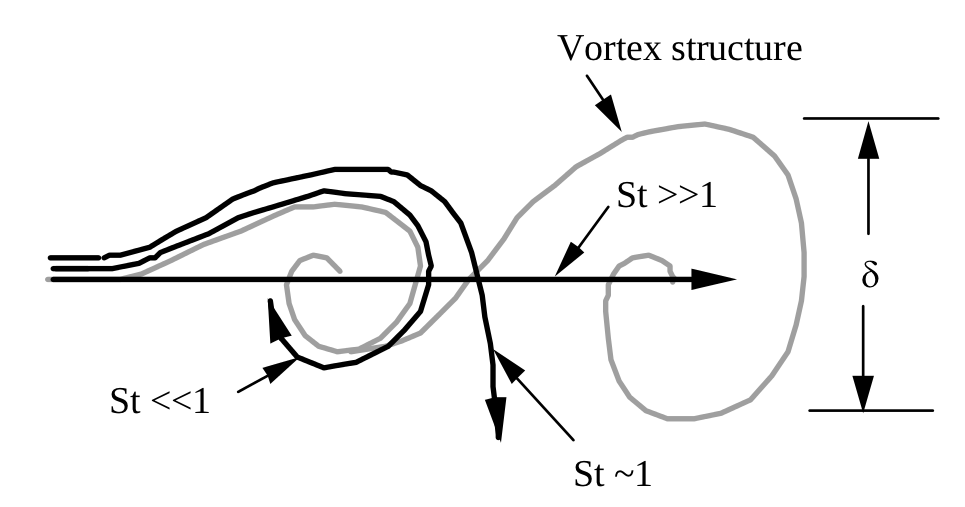
\includegraphics[width=0.75\textwidth]{./figuras/chap1/stokes.png}
\end{tabular}
 \caption{Effect of Stokes number on particle dispersion in large-scale turbulent structures, reproduced from \cite{crowe1988particle}.}
 \label{fig: intro_stokes}
\end{figure}

Apart all the implications concerning a multiphase flow, a spray jet is often turbulent, and the correct prediction of its evolution is dependent on how turbulence is modeled. It was said that the choice of the Lagrangian point-particle method to model the dispersed phase was based on the low liquid volume fraction. A second precaution is also very important when choosing the turbulence modeling for the gaseous flow and the dispersion modeling for the droplets. For spray jets where droplet Stokes number is very low ($St << 1$), see \cite{crowe1988particle} for the definition, the droplets are likely to completely follow oscillations in gas velocity and the interaction with turbulence is strong.

For such sprays, RANS modeling is likely to fail in predicting droplet motion and dispersion\footnote{Dispersion in the context of a spray is used in a similar sense to that in waves. It means that droplet velocity will be significantly dependent on its diameter as wave velocity would be dependent on frequency or wavenumber. } because the interaction with eddies will be restricted to some submodel.  The subject of turbulent dispersed multiphase flow is reviewed by \cite{balachandar2010turbulent} and the most important implications in droplet motion and evaporation are discussed in \cite{sirignano}.

In this work, the jet Reynolds number is not high ($Re=16,300$) and the Stokes number is $\left( St \in [1,100] \right)$ with an average of $10$. It is verified in Chapter \ref{chap: results} that the stochastic subgrid model used together with the traditional k-epsilon model was able to predict some dispersion in droplet velocities.

For the gas phase, it is a known fact that the k-epsilon model must have its coefficients tunned for improved accuracy in predicting the velocity field of a turbulent round jet. However, the exact modifications are not known \textit{a priori} and this work has used the usual coefficients. The consequences of this setup are discussed in Chapter \ref{chap: results}.

% \section{The OpenFOAM code}

% This thesis has made use of moderate computational resources and the open source software OpenFOAM\footnote{OpenFOAM is managed and distributed by the OpenFOAM Foundation and is freely available and open source, licensed under the GNU General Public Licence.}.

\section{Thesis Outline}

Chapter \ref{chap: equations} presents the governing equations for both the continuous and dispersed phases and the type of boundary conditions.
The continuous phase section starts with the fully compressible flow formulation, proceeds with the low Mach number approximation and then the averaging process of the turbulence modeling. The dispersed phase section describes the Lagrangian point-particle method and derives the models for momentum, heat and mass transfer between the droplets and the gas phase. 

Chapter \ref{chap: exp} briefly describes the experiment of \cite{chen}, which was used to evaluate the numerical results. It also presents the boundary conditions for the simulation obtained from the available experimental data.

Chapter \ref{chap: numerical} presents some aspects of the numerical solution such as the equation discretization schemes, the algorithms for solving linear systems and the mesh grid used for the domain discretization.

Chapter \ref{chap: results} presents the results and discussions. The first section presents the results for the properties of the gas phase turbulent jet: the spread rate and the self-similar profiles. The second section presents the results for droplet and gas velocities. The third section presents the mass fluxes of liquid and vapor and the droplet Sauter mean diameter.

Chapter \ref{chap: conclusion} summarizes the conclusions and suggestions for future work.

Appendix \ref{appendix 1} shows the derivation of the conservation equation of sensible enthalpy starting from the total energy equation.

Appendix \ref{appendix 2} show 2D Figures of droplet and gas properties.

Appendix \ref{appendix 3} briefly describes equation discretization and PISO algorithm.


\chapter{Governing Equations}\label{chap: equations}

This chapter presents the governing equations for continuous and dispersed phases.

Continuous phase equations start from the compressible formulation found in \cite{poinsot2005theoretical} with the additional spray source terms. It then proceeds with the low Mach number approximation proposed in \cite{majda}. Finally, the turbulence model is presented with the extra assumptions concerning the turbulent fluxes.

Dispersed phase equations are basically those presented in \cite{nordin} and further discussed in \cite{vonkarman}, \cite{naca} and \cite{baumgarten2006mixture}.

\section{Continuous (Gaseous) Phase}

The continuous phase is the denomination for all gaseous phase in the flow
domain. The set of governing equations is composed by mass, species, momentum, energy
 and state equations. The dispersed phase will
contribute with source/sink terms for each of the gaseous phase equations and extra closure relations
will be used to account for all the phenomena complexity e.g. turbulence and
species diffusion.

All unknowns $(\rho, Y_k, \bv{U}, T)$ are functions of position and time, e.g.
$\bv{U}=\bv{U}(\bv{x},t)$. For notation reduction, however, the function
arguments will be omitted.

\subsection{Fully Compressible Formulation}

The mass (or continuity) equation for a compressible flow with the
spray source term $S_m$ is
\begin{equation}\label{ns: mass}
\frac{\partial \rho}{\partial t} + \nabla \cdot \left( \rho \bv{U} \right) =
S_m \, .
\end{equation}

\begin{remark}Since mass equation is not homogeneous due to the presence
of the spray source term, the traditional
non-conservative form of the equations must be modified. For an intensive
property $\eta$,
\begin{equation}
\begin{split}
 \frac{\partial \rho \eta}{\partial t} + \nabla \cdot \left( \rho \bv{U} \eta
\right) &= \frac{\partial \rho}{\partial t}\eta + \rho\frac{\partial
\eta}{\partial t} + \rho \bv{U} \cdot \nabla \eta + \eta \nabla \cdot \left(
\rho \bv{U} \right) \\
&= \rho \left( \frac{\partial \eta}{\partial t} + \bv{U} \cdot \nabla \eta
\right) + \eta \left[ \frac{\partial \rho}{\partial t} + \nabla \cdot \left(
\rho \bv{U} \right) \right]\\
&= \rho \left( \frac{\partial \eta}{\partial t} + \bv{U} \cdot \nabla \eta
\right) + \eta S_m \, .
\end{split}
\end{equation}
\end{remark}

Species equation with the spray source term $S_{Yk}$ is
\begin{equation}\label{ns: species}
\frac{\partial \rho Y_k }{\partial t} + \nabla \cdot \left( \rho \left( \bv{U} +
\bv{V}_{k}\right) Y_k \right) = S_{Yk} \, ,
\end{equation} where $V_k$ is the diffusion velocity of species $k$ satisfying
$\sum_{k} V_k Y_k = 0$.

The diffusion velocities will be obtained under the approximation of a dilute
mixture in which one of the species has a considerably higher concentration
relative to the others. This is the case for the spray evaporation into an air
atmosphere, where $76.7\%$ of air mass composition is nitrogen.

If $M-1$ species are present in scarce quantities relative to the last species
denoted by $M$, then these $M-1$ species diffuse as in a binary mixture:
\begin{subequations}\label{eq: byndiff}
\begin{align}
V_k Y_k &= -\mathcal{D}_k \nabla Y_k \, , \quad k=1,2,...,M-1 \, ,\\
V_M Y_M &=  \sum_{k=1}^{M-1} \mathcal{D}_k \nabla Y_k \, ,
\end{align}
\end{subequations}
where $\mathcal{D}_k$ is the binary diffusion coefficient of species $k$ and does not need
to be the same for all species.

The scarce species transport equation is then:
\begin{equation}
 \frac{\partial \rho Y_k }{\partial t} + \nabla \cdot\left( \rho Y_k \bv{U}
\right) = \nabla \cdot \left( \rho \mathcal{D}_k\nabla Y_k \right) +S_{Yk}
\, , \quad k=1,2,...,M-1.
\end{equation}


$Y_M$ is obtained from the fact that $\sum_k Y_k =1$,
\begin{equation}
Y_M = 1-\sum_{k=1}^{M-1} Y_k \, .
\end{equation}

The momentum equation is written with the assumption of a compressible Newtonian
fluid \cite{batchelor2000introduction} and includes the gravitational field
$\bv{g}$ and the spray source term $\bv{S}_{mom}$.
\begin{equation}\label{ns: momentum}
\frac{\partial \rho \bv{U} }{\partial t} + \nabla \cdot \left(\rho \bv{U}\bv{U}
\right) = -\nabla p + \nabla \cdot \bv{\tau} +\rho \bv{g}+\bv{S}_{mom} \, ,
\end{equation} where $\bv{\tau}$ is the corresponding viscous stress tensor
\begin{equation}
\bv{\tau} =  2\mu  \left[ \bv{S} -\frac{1}{3} \left( \nabla \cdot \bv{U}
\right)\bv{I} \right]\, ,
\end{equation}
and 
$\bv{S}$ is the strain tensor:
\begin{equation}
\bv{S} = \frac{1}{2} \left( \nabla\bv{U} + \nabla \bv{U}^{T} \right) \, .
\end{equation}

\begin{notation}
 $\nabla \bv{U} = \partial u_i/\partial x_j$ where $u_i$ denotes the
components of $\bv{U}$. Similarly, $\nabla \bv{U}^{T} = \partial
u_j/\partial x_i$. $\bv{I}$ denotes the identity tensor.
\end{notation}

The energy equation might be written in several different forms
(see \cite{poinsot2005theoretical}, chapter 1). Here, the sensible enthalpy
formulation will be preferred. The sensible enthalpy is defined as $h_s = h -
\sum_{k} \Delta h^{0}_{f,k} Y_k = \int_{T_{0}}^{T} c_{p} dT$, where $h$ is the
enthalpy and $\Delta h^{0}_{f,k}$ is the enthalpy of formation of species $k$ at
the reference temperature $T_{0}$.

\begin{equation}\label{ns: energy}
 \frac{\partial \rho h_s}{\partial t} +  \nabla \cdot \left( \rho h_s \bv{U}
\right) = \frac{Dp}{Dt} + \nabla \cdot \bv{J}_s +  \bv{\tau} : \nabla\bv{U} +
 S_{hs}\, ,
 \end{equation}
$S_{hs}$ is the spray enthalpy source term. $\bv{J}_s$ includes heat conduction and the enthalpy
diffusion vector:
\begin{equation}
\bv{J}_s =  \kappa \nabla T - \rho \sum_{k=1}^{M} h_{s,k} \bv{V}_k Y_k \, .
\end{equation}

With the assumptions made for species diffusion in \eqref{eq: byndiff},
$\bv{J}_s$ becomes
\begin{equation}
\bv{J}_s =  \kappa \nabla T + \rho \sum_{k=1}^{M-1} \left( h_{s,k}
-h_{s,M}\right) \mathcal{D}_k \nabla Y_k \, .
\end{equation}

\begin{notation}
 $\tau : \nabla \bv{U}$ reads in tensorial notation as following:
\begin{equation}
 \tau : \nabla \bv{U} = 2\mu\left[ \frac{1}{2} \left( \frac{\partial
u_i}{\partial x_j}+\frac{\partial u_j}{\partial x_i}\right)-\frac{1}{3}\left(
\frac{\partial u_i}{\partial x_i} \right) \delta_{ij} \right]  \frac{\partial
u_i}{\partial x_j} \, ,
\end{equation} $\delta_{ij}$ is the Kronecker delta.
\end{notation}



Constant pressure specific heat capacity for species $k$ is denoted by
$c_{p,k}$. Similarly, constant volume specific heat capacity for species
$k$ is $c_{v,k}$. The same quantities for the gaseous mixture and the
corresponding $\gamma$ constant are then
\begin{subequations}
 \begin{align}
  c_{p} &= \sum_{k} c_{p,k} Y_k \, , \\
  c_{v} &= \sum_{k} c_{p,k} Y_k \, , \\
  \gamma &= c_{p} / c_{v} \, .
 \end{align}
\end{subequations}
The gas mixture is assumed to be an ideal gas mixture and the state equation is
given by
\begin{equation}
 p =  \frac{\gamma -1}{\gamma} \rho c_p T = \frac{1}{W}\rho R T \, ,
\end{equation} where

\begin{equation}
 \frac{1}{W}=\left( \sum_k \frac{Y_k}{W_k} \right) \, .
\end{equation}





\subsection{Non-Dimensional Equations}

All equations may be written in non-dimensional form once
reference quantities are defined.
\begin{itemize}
 \item Distance is given in units of nozzle diameter $D_{jet}$;
 \item Velocity is given in units of average axial velocity
at nozzle exit $\req{U}$;
 \item Time is given in units of $ D_{jet} / \req{U}$;      
 \item Temperature is given in units of ambient temperature $T_{\infty}$;
 \item Pressure is given in units of ambient pressure $p_{\infty}$;
 \item Mass fractions are already non-dimensional;
 \item Molar mass of species k, $W_k$, is given in units of ambient air
molar mass $W_{\infty}$;
 \item Density is given in units of $\rho_{\infty}=p_{\infty} W_{\infty} / R T_{\infty}$;
 \item $c_p$ is given in units of air $c_p$ at conditions $(p_{\infty},T_{\infty})$, or
$c_{p,\infty}$. $\gamma_{\infty}$ is $c_p / c_v$ for the air at the same conditions;
 \item $h_s$ is given in units of $c_{p,\infty} T_{\infty}$.
 \item $\mathcal{D}_k$, $\mu$ and $\kappa$ are given in units of their values at ambient conditions: $\mathcal{D}_{k,\infty}$, $\mu_{\infty}$ and $\kappa_{\infty}$.
 \item $g$ is one unit of the constant gravitational field.
\end{itemize}

The following non-dimensional parameters are also defined:
\begin{subequations}
 \begin{align}
  Re &= \frac{\rho_{\infty} \req{U} D_{jet}}{\mu_{\infty}} \, ,\\
  M  &= \frac{\req{U}}{\sqrt{\gamma_{\infty} R T_{\infty}}}= \frac{\req{U}}{\sqrt{\gamma_{\infty}
  p_{\infty} /\rho_{\infty}}} \, , \\
  Pr &= \frac{\mu_{\infty} c_{p,\infty}}{\kappa_{\infty}} \, , \\
  Le_k &= \frac{\kappa_{\infty}}{\rho_{\infty} c_{p,_{\infty}} \mathcal{D}_{k,\infty}} \, , \\
  Sc_k &= \frac{\mu_{\infty}}{\rho_{\infty} \mathcal{D}_{k,\infty}} = Pr Le_k \, , \\
  Fr &= \frac{\req{U}}{\sqrt{g D_{jet}}} \, .
 \end{align}
\end{subequations}

Equations are then rewritten in terms of non-dimensional quantities.
\begin{description}
\item[State equation:]
\begin{equation}\label{nd: state}
p=\rho T \left( \sum_k \frac{Y_k}{W_k}\right) = \frac{\rho T}{W} \, .
\end{equation}
\item[Mass equation:]
\begin{equation}\label{nd: mass}
\frac{\partial \rho}{\partial t} + \nabla \cdot \left( \rho \bv{U} \right) = 
S_m \, .
\end{equation}
\item[Species equation:]
\begin{subequations}\label{nd: species}
\begin{equation}
 \frac{\partial \rho Y_k }{\partial t} + \nabla \cdot\left(\rho \bv{U} Y_k
\right) = \frac{1}{Re Sc_k} \nabla \cdot \left( \rho \mathcal{D}_k \nabla Y_k
\right) +S_{Yk} \, , \quad k=1,2,...,M-1 \, .
\end{equation}
\begin{equation}
Y_M = 1- \sum_{k=1}^{M-1} Y_k \, .
\end{equation}
\end{subequations}
\item[Momentum equation:]
\begin{equation}\label{nd: momentum}
 \frac{\partial \rho \bv{U} }{\partial t} + \nabla \cdot \left( \rho \bv{U}
\bv{U} \right) = -\frac{1}{\gamma_{\infty} M^2} \nabla p + \frac{1}{Re} \nabla \cdot
\bv{\tau} +\frac{\rho}{Fr^2} \frac{\bv{g}}{|\bv{g}|}+\bv{S}_{mom} \, .
\end{equation} 
\item[Energy equation:]
\begin{equation}\label{nd: enthalpy}
\begin{split}
\frac{\partial \rho h_s}{\partial t} +  \nabla \cdot \left(\rho \bv{U} h_s
\right) &= \frac{\gamma_{\infty} -1}{\gamma_{\infty}}\frac{Dp}{Dt} + \nabla \cdot \bv{J}_s \\
&+ M^2 \left( \gamma_{\infty}-1 \right) \left( \frac{\bv{\tau} : \nabla\bv{U}}{Re}  \right) + S_{hs}\, ,
\end{split}
\end{equation} 
\end{description}

where $\bv{\tau}$ is the shear stress tensor \begin{equation}
\bv{\tau} =  2 \mu \left[ \bv{S} -\frac{1}{3} \left( \nabla \cdot \bv{U}
\right)\bv{I} \right]\, ,
\end{equation}
$\bv{I}$ is the identity tensor and $\bv{S}$ is the strain tensor
\begin{equation}
\bv{S} = \frac{1}{2} \left( \nabla\bv{U} + \nabla \bv{U}^{T} \right) \, .
\end{equation}
$\bv{J}_s$ is the heat conduction and the sensible enthalpy diffusion:
\begin{equation}
\bv{J}_s =  \frac{\kappa}{Re Pr} \nabla T + \sum_{k=1}^{M-1} \frac{\rho
\mathcal{D}_k}{Re Sc_k} \left( h_{s,k} -h_{s,M} \right) \nabla Y_k  \, .
\end{equation}

\subsection{Low Mach Number Approximation}
Consider the following definitions \cite{viozat1997implicit}:

\begin{quote}
A \textbf{compressible flow} is a flow in which density depends on pressure and
temperature.
\end{quote}

\begin{quote}
A \textbf{dilatable flow} is a flow in which density depends on temperature.
\end{quote}

The gas flow considered in this work is fairly incompressible, indeed the
local Mach number is below $0.1$ throughout the flow domain. However, the
intense heat and mass transfers between gaseous and liquid phases when
spray is present produce large temperature gradients which cause density to vary
considerably and the two-phase flow may be classified as a dilatable flow in the
sense of the definition above.

An important difference between incompressible and dilatable flows is
that $\nabla \cdot \bv{U} = 0$ does not hold for the latter. 

A common treatment for dilatable flows is the low Mach number approximation, which consists in expanding unknown quantities $p$, $Y_k$, $\bv{U}$ and $T$ in Equations \eqref{ns:
mass}, \eqref{ns: momentum} and \eqref{ns: energy} into power series
of $\xi \equiv \sqrt{\gamma_{\infty}} M$:
\begin{subequations}\label{eq: expansion}
 \begin{align}
   p &= p_{0} + p_{1}\xi + p_{2}\xi^2 + O\left( \xi^3 \right) \, ,\\
   Y_k &= Y_{k,0} + O\left( \xi \right) \, ,\\
  \bv{U} &= \bv{U}_{0} + O\left( \xi \right) \, ,\\
  T &= T_{0} + O\left( \xi \right) \, .
 \end{align}
\end{subequations}

The reason for expanding pressure up to the second order while keeping only the
leading (or zeroth) order for the other variables is discussed in
\cite{muller1999low}, but it is essentially because of the $M^{-2}$ factor in momentum equation \eqref{nd: momentum}. 

The dependence of the spray source terms on the flow variables is also considered only for the leading order.

$\rho_0$ is obtained by substitution of \eqref{eq: expansion} into the
non-dimensional state equation. $\rho_0$ is such that
\begin{equation}\label{lm: state}
 p_0 = \rho_0 T_0 \left( \sum_k \frac{Y_{k,0}}{W_k} \right) =  \frac{ \rho_0
T_0}{W_0}\, .
\end{equation}

Mass equation \eqref{nd: mass} of order $\xi^0$ becomes:
\begin{equation}
 \frac{\partial \rho_0}{\partial t} + \nabla \cdot \left( \rho_0 \bv{U}_0
\right) =  S_m \, .
\end{equation}

Species equation \eqref{nd: species} of order $\xi^0$ is:
\begin{subequations}\label{lm: species}
\begin{align}
 \frac{\partial \rho_0 Y_{k,0} }{\partial t} + \nabla \cdot\left(\rho_0 \bv{U}_0
Y_{k,0} \right) &= \frac{1}{Re Sc_k} \nabla \cdot \left( \rho \mathcal{D}_k
\nabla Y_{k,0} \right) +S_{Yk} \, , \quad k=1,2,...,M-1 \, . \\
  Y_{M,0} &= 1- \sum_{k=1}^{M-1} Y_{k,0} \, .
\end{align}
\end{subequations}

The momentum equation gives information of orders $\xi^{-2}$, $\xi^{-1}$ and
$\xi^0$ due to the presence of the coefficient $1/\xi^2$ in the pressure gradient . The
resulting equations are, respectively,
\begin{subequations}\label{lm: momentum}
\begin{align}
 \nabla p_0 &\equiv 0 \, , \\
 \nabla p_1 &\equiv 0 \, , \\
 \frac{\partial \rho_0 \bv{U}_0 }{\partial t} + \nabla \cdot \left( \rho_0
\bv{U}_0 \bv{U}_0 \right) &= -\nabla p_2 + \frac{1}{Re} \nabla \cdot \bv{\tau}_0
+\frac{\rho_0}{Fr^2} \frac{\bv{g}}{|\bv{g}|}+\bv{S}_{mom}  \, .
\end{align}
\end{subequations}

From $\nabla p_0 \equiv \nabla p_1 \equiv 0$, it is observed that $p_0$ and
$p_1$ are functions of time only, $p_0 = p_0 (t)$ and $p_1 = p_1 (t)$. The
coupling between  velocity and pressure fields is now separated into two
contributions:  $p_2$ establishes the pressure gradient and will be referred to
as the dynamic pressure; $p_0$ affects $\rho_0$ via the state equation and will
be referred to as the thermodynamic pressure. 

The energy equation reads
\begin{equation}\label{lm: enthalpy}
\frac{\partial \rho_0 h_{s0}}{\partial t} +  \nabla \cdot \left(\rho_0 \bv{U}_0
h_{s0} \right) = \frac{\gamma_{\infty} -1}{\gamma_{\infty}}\frac{Dp_0}{Dt} + \nabla \cdot
\bv{J}_{s0} + S_{hs}\, ,
\end{equation} where 
\begin{equation}
\bv{J}_{s0} =  \frac{\kappa}{Re Pr} \nabla T_0 + \sum_{k=1}^{M-1}
\frac{\rho\mathcal{D}_k}{Re Sc_k} \left( h_{s0,k} -h_{s0,M} \right) \nabla
Y_{k,0} \, . 
\end{equation}

An ordinary differential equation in time may be derived for computing the thermodynamic pressure ($p_0$) by differentiating the state equation \eqref{lm: state} with respect to time and integrating in domain volume:
\begin{equation}\label{lm: dstate}
 \frac{Dp_0}{Dt}\int_{\Omega}W dV + p_0 \int_{\Omega}\frac{DW}{Dt} dV=\int_{\Omega} \frac{D\rho T}{Dt} dV\, ,
\end{equation}
where 
\begin{equation}
\frac{D}{Dt} = \frac{\partial}{\partial t}+\bv{U}\cdot\nabla
\end{equation}
is the total derivative.

Each total derivative may be computed from mixture molar mass ($W$) definition and mass, species and enthalpy equations. 

For an infinite (or open) domain $\Omega$, 
\begin{equation}
\int_{\Omega}\frac{DW}{Dt} dV < \infty \, , \quad \int_{\Omega} \frac{D\rho T}{Dt} dV < \infty \quad \text{and} \quad \int_{\Omega}W dV = \infty \, .
\end{equation}
 Hence, $Dp_0/Dt = 0$ and $p_0 = 1$, the non-dimensional pressure in far-field boundary.

Herein, the subscripts denoting the order of expansion will be omitted, except
for the pressure. $\bv{U}_0$ is simply $\bv{U}$ and the same holds to $\rho$,
$Y_k$, $h_s$ and $T$. For pressure, $p_0$ is the thermodynamic pressure and
$p_2$ is the dynamic pressure.

\subsection{Turbulence Modeling}

The expression \textit{turbulent and evaporating spray} entitling this work
refers to a liquid spray evolving in a gaseous turbulent flow where mass, energy
and momentum transfers between both phases are strongly affected by turbulence. 

Among all possible treatments for turbulent flows, see
\cite{pope2000turbulent}, one is perhaps the most widely used in industrial
applications: the so called \textit{standard k-epsilon model}. This two-equation
model within the RANS (Reynolds-averaged Navier-Stokes) framework provides a good
compromise between complexity and computational cost for those not using
exceptional computational resources. 

In the context of RANS modeling, the governing equations are averaged and solved
for the mean values of flow properties. The effect of turbulence on the mean
field is accounted by modeling the terms depending on the fluctuations. In the
specific case of the momentum equation, the hypothesis of turbulent-viscosity
(or Boussinesq hypothesis) is used to compute an effective value of local
viscosity composed by molecular and turbulent viscosities, being the
latter an approximation of the extra momentum flux of Reynolds stresses.

For compressible flows, two averages are commonly used: the simple time average
and a mass-weighted time average (or Favre average), see \cite{favre1969statistical}.
The time average $(\bar{f})$ and the deviation $(f')$  of a quantity $f$ are
defined as
\begin{equation}
 \bar{f}(x,t) \equiv \frac{1}{T}\int_{t}^{t+T} f(x,\tau) d\tau \quad \text{and}
\quad f'(x,t)= f(x,t)-\bar{f}(x,t) \, .
\end{equation}

The mass-weighted average (or Favre average) $(\tilde{f})$ and the deviation
$(f'')$ are defined as
\begin{equation}
 \tilde{f}(x,t) = \frac{\overline{\rho f(x,t)}}{\bar{\rho}} \quad \text{and}
\quad f^{''}(x,t) = f(x,t) - \tilde{f}(x,t) \, .
\end{equation}

Following the definitions,
\begin{equation}
 \quad \overline{f'}=\bar{f}-\bar{f}=0 \quad \text{and} \quad \bar{\bar{f}}=
\bar{f}\, ,
\end{equation}
\begin{equation}
 \quad \tilde{f''}=\tilde{f}-\tilde{f}=0 \quad \text{and} \quad \tilde{\tilde{f}}=
\tilde{f}\, .
\end{equation}
Averaging and differential operators are assumed to commute, see \cite{pope2000turbulent}. 

\subsubsection{Mass and Species Equations}
Averaged mass and species equations are easily obtained. The
averaged mass equation reads:
\begin{equation}\label{av: mass}
  \frac{\partial \bar{\rho}}{\partial t} + \nabla \cdot \left( \bar{\rho}
\tilde{\bv{U}} \right) =  \bar{S}_m \, .
\end{equation}

The species averaged equation reads:
\begin{subequations}\label{av: species1}
\begin{equation}
 \frac{\partial \bar{\rho} \tilde{Y}_k }{\partial t} + \nabla
\cdot\left(\bar{\rho} \tilde{\bv{U}} \tilde{Y}_k +\bar{\rho}\widetilde{\bv{U''}
Y''_{k}} \right) = \frac{1}{Re Sc_k} \nabla \cdot \left( \overline{\rho
\mathcal{D}_k \nabla Y_k} \right) +\bar{S}_{Yk} \, , \quad k=1,2,...,M-1 \, ,
\end{equation}
\begin{equation}
\tilde{Y}_M = 1- \sum_{k=1}^{M-1} \tilde{Y}_{k} \, .
\end{equation}
\end{subequations}
Equation \eqref{av: species1} shows two new terms: $\overline{\rho \mathcal{D}_k \nabla
Y_k}$ and $\bar{\rho}  \widetilde{\bv{U}'' Y_k^{''}}$. Unless new equations are
derived for them, both terms are not known and must be modeled.

For the first one, regarding the laminar diffusivity of species, the average is
commonly approximated as shown below:
\begin{equation}
\overline{\rho \mathcal{D}_k \nabla Y_k} \approx \bar{\rho}\mathcal{D}_k \nabla
\tilde{Y}_k \, .
\end{equation}

For the second term, which deals with turbulent flux, an approach analogous
to turbulent-viscosity is used and a turbulent coefficient for species
diffusion $(\mathcal{D}_{k,t})$ is used:
\begin{equation}
\bar{\rho}  \widetilde{\bv{U}'' Y_k^{''}} \approx -\frac{\bar{\rho}
\mathcal{D}_{k,t}}{Re Sc_k} \nabla \tilde{Y}_k \, ,
\end{equation}
$\mathcal{D}_{k,t}$ is computed by the turbulence model.

The species equation then becomes:
\begin{subequations}\label{av: species}
\begin{equation}
 \frac{\partial \bar{\rho} \tilde{Y}_k }{\partial t} + \nabla
\cdot\left(\bar{\rho} \tilde{\bv{U}} \tilde{Y}_k \right) = \frac{1}{Re Sc_k}
\nabla \cdot \left[ \bar{\rho} \left( \mathcal{D}_k + \mathcal{D}_{k,t} \right)
\nabla \tilde{Y}_k \right] +\bar{S}_{Yk} \, , \quad k=1,2,...,M-1 \, .
\end{equation}
\begin{equation}
\tilde{Y}_M = 1- \sum_{k=1}^{M-1} \tilde{Y}_{k} \, .
\end{equation}
\end{subequations}

\subsubsection{Momentum Equation}
Treatment of momentum equation is more complicated and it is shown in more
steps here. The averaged momentum equation reads:
\begin{equation}
 \frac{\partial \bar{\rho} \tilde{\bv{U}} }{\partial t} + \nabla \cdot \left(
\bar{\rho} \tilde{\bv{U}} \tilde{\bv{U}} \right) = -\nabla \bar{p}_2 +  \nabla
\cdot \left(  \frac{\bar{\bv{\tau}}}{Re} - \bar{\rho}\widetilde{\bv{U}''
\bv{U}''} \right) +\frac{\bar{\rho}}{Fr^2}
\frac{\bv{g}}{|\bv{g}|}+\bar{\bv{S}}_{mom}  \, .
\end{equation}

Again, two terms are new and unknown: $\bar{\tau}$ and $-
\bar{\rho}\widetilde{\bv{U}'' \bv{U}''}$. From the definitions of averages, 
\begin{equation}
 \tau = \tilde{\tau}+\tau'' \quad \Rightarrow \quad \bar{\tau} =
\tilde{\tau}+\overline{\tau''} \, ,
\end{equation}
and assuming $\tilde{\tau} \gg \overline{\tau''}$, we have:
\begin{equation}
 \bar{\tau} \approx  2\mu\left[ \tilde{S}-\frac{I}{3}\left(\nabla \cdot
\tilde{\bv{U}} \right)  \right] \, .
\end{equation}

The modeling of the turbulent momentum flux is made by the following
expression (known as Boussinesq hypothesis):
\begin{equation}\label{eq: boussinesq}
 - \bar{\rho}\widetilde{\bv{U}'' \bv{U}''} =  \frac{2 \mu_t}{Re} \left[
\tilde{S}-\frac{I}{3} \left( \nabla \cdot \tilde{\bv{U}} \right)  \right] -
\frac{2}{3}\bar{\rho}kI \, .
\end{equation}

$\mu_t$ is the turbulent-viscosity accounting for the extra momentum flux due to the Reynolds stresses ($-
\bar{\rho}\widetilde{\bv{U}'' \bv{U}''}$). $k$ is turbulent kinetic energy defined as:
\begin{equation}
  k = \frac{1}{2} \widetilde{\left(\bv{U}'' \cdot \bv{U}'' \right) \, .}
\end{equation}
Both $\mu_t$ and $k$ are computed by the turbulence model.

$\tau_{tot}$ is defined as a ``new viscous stress tensor'' composed by the
laminar and turbulent part:
\begin{equation}
 \overline{\tau_{tot}} \equiv 2 (\mu + \mu_t) \left[
\tilde{S}-\frac{I}{3}\left(\nabla \cdot \tilde{\bv{U}} \right)  \right]
-\frac{2}{3}\bar{\rho}k I \, ,
\end{equation}
and the momentum equation finally becomes:
\begin{equation}\label{av: momentum}
 \frac{\partial \bar{\rho} \tilde{\bv{U}} }{\partial t} + \nabla \cdot \left(
\bar{\rho} \tilde{\bv{U}} \tilde{\bv{U}} \right) = -\nabla \bar{p}_2 +  
\frac{1}{Re}  \nabla \cdot\overline{\bv{\tau}_{tot}} +\frac{\bar{\rho}}{Fr^2}
\frac{\bv{g}}{|\bv{g}|}+\bar{\bv{S}}_{mom}  \, .
\end{equation}

\subsubsection{Sensible Enthalpy Equation}
The averaged sensible enthalpy equation reads:
\begin{equation}
\frac{\partial \bar{\rho} \tilde{h}_{s}}{\partial t} + \nabla \cdot
\left(\bar{\rho} \tilde{\bv{U}} \tilde{h}_{s} + \bar{\rho} \widetilde{\bv{U}''
h_s^{''}} \right) = \frac{\gamma_{\infty} -1}{\gamma_{\infty}}\overline{\frac{Dp_0}{Dt}} + \nabla
\cdot \bar{\bv{J}}_s + \bar{S}_{hs}\, ,
\end{equation} where 
\begin{equation}
\bv{J}_s =  \overline{\frac{\kappa}{Re Pr} \nabla T} + \sum_{k=1}^{M-1}
\overline{\frac{\rho\mathcal{D}_k}{Re Sc_k} \left( h_{s,k} -h_{s,M} \right)
\nabla Y_{k}} \, . 
\end{equation}

Four new terms are unknown and must be modeled as well:\\  $\bar{\rho}
\widetilde{\bv{U}'' h_s^{''}} $ , $\overline{\frac{Dp}{Dt}} $, 
$\overline{\frac{\kappa}{Re Pr} \nabla T}$ and 
$\overline{\frac{\rho\mathcal{D}_k}{Re Sc_k} \left( h_{s,k} -h_{s,M} \right)
\nabla Y_{k}} $.

Turbulent flux of enthalpy is modeled similarly to species and momentum
turbulent fluxes:
\begin{equation}
 \bar{\rho} \widetilde{\bv{U}'' h_s^{''}} \approx -\frac{\bar{\rho} \alpha_t
}{Re Pr} \nabla \tilde{h}_s \, ,
\end{equation}
where $\alpha_t$ is the turbulent thermal diffusivity that is also computed by the
turbulence model.

The average of the total derivative $\overline{Dp/Dt}$ reads:
\begin{equation}
 \overline{\frac{D p_0}{D t}} = \frac{\partial \bar{p}_0}{\partial
t}+\overline{\bv{U} \cdot \nabla p_0} = \frac{\partial \bar{p}_0}{\partial t} + \left( \tilde{\bv{U}} \cdot \nabla \bar{p}_0 \right) + \overline{\bv{U}'' \cdot \nabla p_0}
\end{equation}
Neglecting the last term ($\overline{\bv{U}'' \cdot \nabla p_0}$) gives:
\begin{equation}
 \overline{\frac{D p_0}{D t}}  \approx \frac{\partial \bar{p}_0}{\partial t} +
\left( \tilde{\bv{U}} \cdot \nabla \bar{p}_0 \right)\, .
\end{equation}

For laminar heat diffusion, the effect of fluctuations is neglected and only
averaged terms are considered:
\begin{equation}
 \overline{k \nabla T} = \bar{k} \nabla \tilde{T} + \overline{k\nabla T''}
\approx \bar{k} \nabla \tilde{T} \, .
\end{equation} 

Under the same assumption:
\begin{equation}
 \overline{\frac{\rho \mathcal{D}_k}{Re Sc_k}\left( h_{s,k} - h_{s,M} \right)
\nabla Y_k} \approx \frac{\bar{\rho} \mathcal{D}_k}{Re Sc_k} \left[ \left( \tilde{h}_{s,k} -
\tilde{h}_{s,M }\right) \nabla \tilde{Y}_k \right] \, .
\end{equation}

Sensible enthalpy equation finally becomes:
\begin{equation}\label{av: enthalpy}
\frac{\partial \bar{\rho} \tilde{h}_{s}}{\partial t} + \nabla \cdot
\left(\bar{\rho} \tilde{\bv{U}} \tilde{h}_{s} \right) = \frac{\gamma_{\infty} -1}{\gamma_{\infty}}
\left[ \frac{\partial \bar{p}_0}{\partial t} + \left( \tilde{\bv{U}} \cdot \nabla
\bar{p}_0 \right) \right]  + \nabla \cdot \bar{\bv{J}}_s + \bar{S}_{hs}\, ,
\end{equation} where 
\begin{equation}
\bar{\bv{J}}_s =  \frac{\bar{\rho} \left( \alpha + \alpha_t \right)}{Re Pr}
\nabla \tilde{h}_s + \sum_{k=1}^{M-1} \frac{\rho \mathcal{D}_k}{Re Sc_k} \left[
\left( \tilde{h}_{s,k} - \tilde{h}_{s,M }\right) \nabla \tilde{Y}_k \right] \, .
\end{equation}

All unclosed terms are now specified if the following parameters are given by
the turbulence model:
\begin{equation*}
 k, \quad \mu_t , \quad \alpha_t , \quad \mathcal{D}_{k,t} \, .
\end{equation*}

Further assumptions are made: 

\begin{itemize}
 \item Unity Schmidt and Prandtl numbers ($Sc_k = Pr = 1$) everywhere in the
flow domain for laminar and turbulent fluxes:
\begin{equation}\label{eq: sc1}
 \bar{\rho} \left(\mathcal{D}_k +\mathcal{D}_{k,t} \right) = \bar{\rho} \left(\alpha +\alpha_{k,t} \right) = \mu+\mu_t \, .
\end{equation} 
Now, the turbulence model only needs to provide $k$ and $\mu_t$.

 \item All species have the same sensible enthalpy:

\begin{equation}
 \sum_{k=1}^{M-1} \frac{\rho \mathcal{D}_k}{Re Sc_k} \left[ \underbrace{\left(
\tilde{h}_{s,k} - \tilde{h}_{s,M }\right)}_{\approx 0} \nabla \tilde{Y}_k
\right] =  0 \, .
\end{equation}

\end{itemize}

\subsubsection{State Equation}

Averaged state equation reads:
\begin{equation}
\overline{p W} = R \overline{\left( \rho T \right)} = R \bar{\rho} \tilde{T} \, ,
\end{equation}
where $1/W = \sum_k Y_k/W_k$.

The term on the rhs - $\overline{p W}$ - is simply approximated as
\begin{equation}
\overline{p W} = \bar{p}\tilde{W}+\overline{p W''} \approx \bar{p}\tilde{W} \, .
\end{equation}

\subsubsection{Relation of Averaged Enthalpy and Temperature}

An expression is needed to relate $\tilde{h}_s$, which is being solved for in Equation \eqref{av: enthalpy}, to Favre-averaged temperature ($\tilde{T}$). From the definition of $h_s$:
\begin{equation}
\tilde{h}_s =\frac{\overline{\rho h_s}}{\bar{\rho}} = \frac{1}{\bar{\rho}}\overline{\left[ \rho \left( \int_{T_0}^{T} \sum_k c_{p,k}(T) dT \right)\right] }.
\end{equation}

Using $c_p=\sum_k c_{p,k} Y_k$, $\ Y_k = \tilde{Y}_k + Y_{k}^{''}$ and $T = \tilde{T}+ T^{''}$, a tricky expression is obtained:
\begin{equation}
\tilde{h}_s = \frac{1}{\bar{\rho}} \overline{\left(\bar{\rho}+\rho' \right) \int_{T_0}^{\tilde{T}+T''} \sum_k c_{p,k} \left(\tilde{T}+ T^{''}\right) \left(\tilde{Y}_k+Y^{''}_k \right) dT} \, .
\end{equation}

A convenient simplification is to simply neglect all fluctations and consider the following approximation:
\begin{equation}
\tilde{h}_s \approx \int_{T_0}^{\tilde{T}} \sum_k c_{p,k}(\tilde{T})\ \tilde{Y}_k\ dT \, .
\end{equation}

\subsubsection{Standard k-epsilon Turbulence Model}

According to the simplification of unity Schmidt and Prandtl numbers made in Equation \eqref{eq: sc1}, the turbulence modeling
is complete once $k$ and $\mu_t$ are specified. The \textit{standard k-epsilon}
model provides one algebraic equation for $\mu_t$ and two differential equations
for $k$ and $\epsilon$, the dissipation rate of $k$. 

\begin{equation}
 \mu_t = \bar{\rho} C_{\mu} \frac{k^2}{\epsilon} \, ,
\end{equation}

\begin{equation}
 \frac{\partial \bar{\rho}k}{\partial t} + \nabla \cdot \left( \bar{\rho}
\tilde{\bv{U}} k \right) = \frac{1}{Re}\nabla \cdot \left[ \left( \mu +
\frac{\mu_t}{\sigma_k} \right) \nabla k \right] -\frac{2}{3} \bar{\rho} k \left(
\nabla \cdot \tilde{\bv{U}} \right) + P_k -\bar{\rho} \epsilon \, ,
\end{equation}

\begin{equation}\begin{split}
 \frac{\partial \bar{\rho}\epsilon}{\partial t} + \nabla \cdot \left( \bar{\rho}
\tilde{\bv{U}} \epsilon \right) = \frac{1}{Re} \nabla \cdot \left[ \left( \mu +
\frac{\mu_t}{\sigma_{\epsilon}} \right) \nabla \epsilon \right]  - \left(
\frac{2}{3}C_{\epsilon1}+C_{\epsilon3}\right)\bar{\rho}\epsilon \left( \nabla
\cdot \tilde{\bv{U}}\right) \\
+ C_{\epsilon 1} \frac{\epsilon}{k} P_k - C_{\epsilon 2} \bar{\rho}
\frac{\epsilon^2}{k} \, ,
\end{split}\end{equation}
where $P_k = - \bar{\rho} \widetilde{\bv{U}'' \bv{U}''}: \nabla \tilde{\bv{U}}$.
The approximation for the term $- \bar{\rho} \widetilde{\bv{U}'' \bv{U}''}$ was
already defined in \eqref{eq: boussinesq} and is repeated here for convenience:

\begin{equation}
 - \bar{\rho}\widetilde{\bv{U}'' \bv{U}''} =  \frac{2 \mu_t}{Re} \left[
\tilde{S}-\frac{I}{3} \left( \nabla \cdot \tilde{\bv{U}} \right)  \right] -
\frac{2}{3}\bar{\rho}kI \, .
\tag{\ref{eq: boussinesq}}
\end{equation}

The model has six parameters whose values are shown in Table \ref{table:
kepscoeff}.
\begin{table}
\centering
 \begin{tabular}{cccccc}
  \hline
  $C_{\mu}$ & $C_{\epsilon 1}$ & $C_{\epsilon 2}$ & $C_{\epsilon 3}$  & $\sigma_k$ & $\sigma_{\epsilon}$\\
  $0.09$ & $1.44$ & $1.92$ & $-0.33$ & $1$ & $1.3$ \\ \hline
 \end{tabular}
\caption{k-epsilon model constants.}
\label{table: kepscoeff}
\end{table} 

It must be pointed out that the droplet dispersion due to turbulence will be modeled in the dispersed phase description. 
However, no sink of turbulent kinetic energy was defined here due to the work done by the eddies on the droplets. 

\subsection{Boundary Conditions}

Four distinct boundary regions are present in the experiment of Chen, St\aa{}rner and Masri:
 nozzle inlet ($\partial \Omega_{nozzle}$), co-flow inlet ($\partial \Omega_{\text{co-flow}}$), far-field boundaries ($\partial \Omega_{\infty}$) and outlet ($\partial \Omega_{outlet}$), see Figure \ref{fig: jet_bc}.

% The prescribed conditions are zero gradient for pressure and fixed values for the remaining unknowns. In the far-field boundaries, pressure is the atmosphere and the other unknowns have a zero gradient condition. In the outlet, zero gradient is specified for all variables.

\begin{description}
 \item[Nozzle inlet conditions:]
\begin{subequations}
 \begin{align}
  \frac{\partial p}{\partial \bv{n}}(\partial \Omega_{nozzle},t)  = 0 \\
  \bv{U}(\partial \Omega_{nozzle},t) = \bv{U}_{nozzle}\left(\bv{x}\right) \\
  T(\partial \Omega_{nozzle},t) = T_{nozzle} \\
  Y_k(\partial \Omega_{nozzle},t) = Y_{k,nozzle}
 \end{align}
\end{subequations}

\item[Coflow conditions:]
\begin{subequations}
 \begin{align}
  \frac{\partial p}{\partial n}(\partial \Omega_{\text{co-flow}},t)  = 0 \\
  \bv{U}(\partial \Omega_{\text{co-flow}},t) = \bv{U}_{\text{co-flow}} \\
  T(\partial \Omega_{\text{co-flow}},t) = T_{\text{co-flow}} \\
  Y_k(\partial \Omega_{\text{co-flow}},t) = Y_{k,\text{co-flow}}
 \end{align}
\end{subequations}

\item[Far-field boundaries:]
\begin{subequations}
 \begin{align}
  p \left( \Omega_b,t \right) &= 1 \\ % non-dimensional value
  \frac{\partial \bv{U}}{\partial \bv{n}} (\partial \Omega_b,t) &= 0 \\
  \frac{\partial T}{\partial \bv{n}} (\partial \Omega_b,t) &= 0 \\
  \frac{\partial Y_k}{\partial \bv{n}}(\partial \Omega_b,t) &= 0 
 \end{align}
\end{subequations}

\item[Outlet conditions:]
\begin{subequations}
 \begin{align}
  \frac{\partial p}{\partial n}(\partial \Omega_{outlet},t)  &= 0 \\
  \frac{\partial \bv{U}}{\partial \bv{n}} (\partial \Omega_{outlet},t) &= 0 \\
  \frac{\partial T}{\partial \bv{n}} (\partial \Omega_{outlet},t) &= 0 \\
  \frac{\partial Y_k}{\partial \bv{n}}(\partial \Omega_{outlet},t) &= 0 
 \end{align}
\end{subequations}
 \end{description}
where $\bv{n}$ is the unit vector normal to the boundary.

Function $\bv{U}_{nozzle}(\bv{x})$ and scalars $T_{nozzle}$, $Y_{k,nozzle}$, $\bv{U}_{\text{co-flow}}$, $T_{\text{co-flow}}$ and $Y_{k,\text{co-flow}}$ are determined in Chapter \ref{chap: exp} from available experimental data.

\begin{figure}
\begin{center}
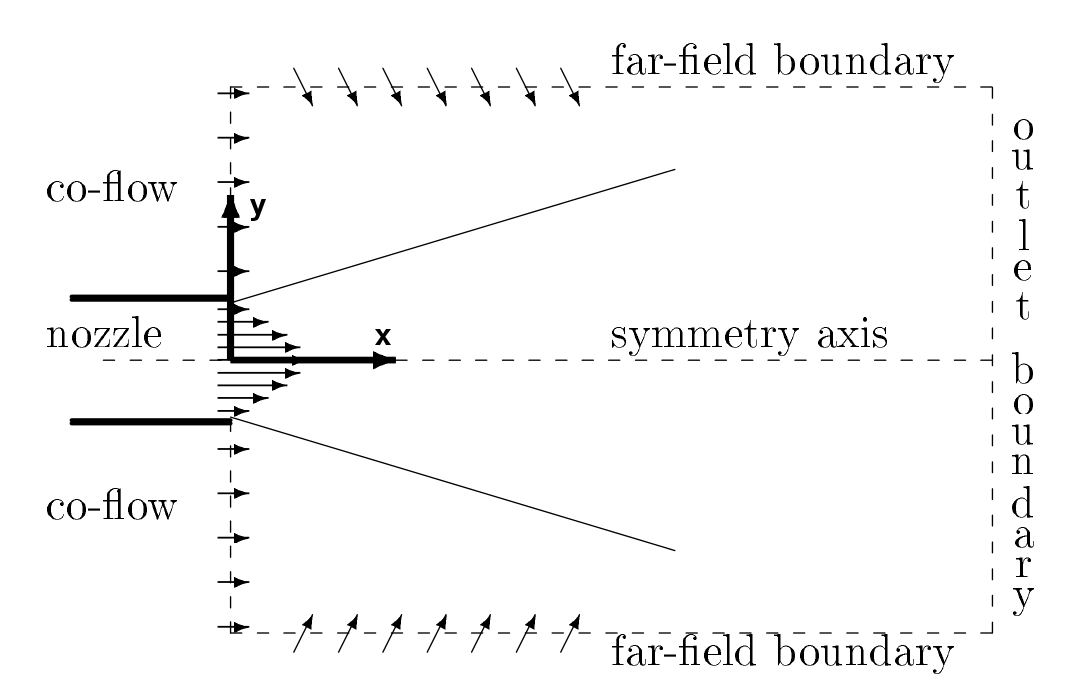
\includegraphics[width=0.75\textwidth]{./figuras/chap2/jet.png}
\end{center}
\caption{Definition of axis orientation and domain boundaries for the emerging round jet flow. Adapted from \cite{luppes}.}
\label{fig: jet_bc}
\end{figure}

Numerical solution of the equations will be performed time accurately due to the stochastic modeling of liquid atomization, as explained later in the dispersed phase section of this chapter. The initial conditions would then be the steady state solution of a pure gas jet. 

The time-dependence of thermodynamic pressure $p_0$ is neglected and it is assumed constantly equal to ambient pressure, or an unity value in dimensionless form,
\begin{equation}
 p_0 (t) = 1 \, .
\end{equation}


\subsubsection{Boundary Conditions of Turbulent Quantities}

Introduction of two new variables in the turbulence model, namely $k$ and $\epsilon$, requires the definition of their boundary conditions.

\begin{description}
 \item[Nozzle inlet conditions:]
\begin{subequations}
 \begin{align}
  k(\partial \Omega_{nozzle},t) &= k_{nozzle}(\bv{x}) \, ,\\
  \epsilon(\partial \Omega_{nozzle},t) &= \epsilon_{nozzle}(\bv{x}) \, ,
 \end{align}
\end{subequations}

\item[Co-flow conditions:]
\begin{subequations}
 \begin{align}
  k(\partial \Omega_{\text{co-flow}},t) &= k_{\text{co-flow}} \, , \\
  \epsilon(\partial \Omega_{\text{co-flow}},t) &= \epsilon_{\text{co-flow}} \, ,
 \end{align}
\end{subequations}

\item[Far-field boundaries:]
\begin{subequations}
 \begin{align}
  \frac{\partial k}{\partial \bv{n}} (\partial \Omega_b,t) &= 0 \, , \\
  \frac{\partial \epsilon}{\partial \bv{n}} (\partial \Omega_b,t) &= 0 \, ,
 \end{align}
\end{subequations}

\item[Outlet conditions:]
\begin{subequations}
 \begin{align}
  \frac{\partial k}{\partial \bv{n}} (\partial \Omega_{outlet},t) &= 0 \, , \\
  \frac{\partial \epsilon}{\partial \bv{n}} (\partial \Omega_{outlet},t) &= 0 \, .
 \end{align}
\end{subequations}
\end{description}

Functions $k_{nozzle}(\bv{x})$ and $\epsilon_{nozzle}(\bv{x})$ and scalars $k_{\text{co-flow}}$ and $\epsilon_{\text{co-flow}}$ are also determined in Chapter \ref{chap: exp}.

\section{Dispersed (Liquid) Phase}

The modeling presented for the liquid phase here is solely intended to deal with
the situation of a narrow liquid jet emerging from a nozzle in a coaxial gaseous
flow in 
specific conditions that cause the liquid jet to atomize, that is, to
disintegrate into a large number of non-contiguous small volumes called
droplets. 
Despite that, this situation is further simplified to produce results for
engineering problems and many of the physical complexities are not addressed.

The ensemble of droplets originated from atomization is called the spray.
The spray evolution in time is a complex phenomenon as the liquid droplets exchange heat, mass
and momentum with the surrounding gas and other droplets. The droplets
also have their inner thermodynamics and might become unstable to the
point where they subdivide into smaller ones.

Here, the droplets will be treated as particles with the following properties:
\begin{itemize}
 \item liquid substance: according to which the constitutive properties will be
defined (only single-component liquids are concerned, see
\cite{baumgarten2006mixture});
 \item geometric properties: all droplets are assumed to be spheric with 
diameter $D$;
 \item thermodynamic properties: pressure, volume, mass, temperature;
 \item kinematic properties: position and velocity (translational only).
\end{itemize}

This description is often called the point-particle method, see \cite{balachandar2010turbulent}.

The next subsections will describe the processes being modeled for
computation of spray evolution (the evolution of all droplet properties in time). 

The approach to the inter-phase interaction shown below is usually called the two-way coupling because it
comprises the interaction between gas and droplet but neglects the interactions between two different droplets, like
droplet collisions. It is mostly used for the case of dilute sprays, when the liquid volumetric fraction ($\phi_{v,l}$) satisfies $\phi_{v,l}<10^{-3}$.

\subsection{Atomization or Primary Break-Up}

The atomization is not modeled in a deterministic way, with the dynamics of liquid jet disintegration into droplets. 

Rather, it is used a stochastic approach called the Monte Carlo's method, see \cite{baumgarten2006mixture}, that describes resulting droplets from atomization process based on available measurements near the nozzle exit plane.

Droplets are inserted into the domain in groups called parcels. A parcel is
a group of droplets with all properties being exactly the same.
This means that one single set of ordinary differential equations is solved for
the entire group (and
not one set for each droplet) the only difference being that the parcel mass ($m_{parcel}$) is
the sum of all droplet mass ($m_d$). This means that,
\begin{equation}
 m_{parcel} = N_d m_d = N_d\left( \rho_d \frac{\pi D^3}{6}\right) \, ,
\end{equation}
where $m_d$ is the droplet mass, $N_d$ is the number of droplets represented by this parcel and $D$ is the parcel (and the droplet) diameter.


For each time instant, a certain number of parcels is inserted into the domain to represent the
liquid injection. The parcel properties in the nozzle exit are specified as either constant values or random variables sampled from statistical distributions built from experimental data.

In this work, all parcel properties in the nozzle have constant values except for the parcel diameter,
which is a random variable.


\subsection{Secondary Break-Up}

The secondary break-up of droplets is neglected. It is considered that droplets
vaporize (and either disappear or have their diameter reduced) before they
become unstable.

\subsection{Momentum Transfer}

The motion and momentum equations for a particle are:
\begin{equation}\label{eq: drop_mom}
\frac{d\bv{x}_d}{dt} =\bv{U}_d  , \quad m_d \frac{d\bv{U}_d}{dt} = \bv{F} \, .
\end{equation}

The resulting force ($\bv{F}$) on the particle  proposed by \cite{vonkarman} is here
simplified for the case of a rigid spheric droplet under small pressure
gradient and in low droplet Reynolds number. The buoyancy force is
neglected because the gas density is much lower than the liquid density ($\rho \ll \rho_d $).  The effect of mass transfer on the droplet momentum equation was also neglected so that
\begin{equation}
 \frac{d \left(m_d \bv{U}_d \right) }{dt}\approx  m_d\frac{d \bv{U}_d }{dt} \, .
\end{equation}


The droplet slip velocity (the droplet velocity relative to the gas) is given by:
\begin{equation}\label{eq: Urel}
 \bv{U}_{slip} = \bv{U_d} - \underbrace{\left( \tilde{\bv{U}}+\bv{U}'' \right)}_{\text{gas}} \, ,
\end{equation}
where $\tilde{\bv{U}}$ is the Favre-averaged gas velocity computed in Equation \eqref{av: momentum} and $\bv{U}''$ is its fluctuation.
Since $\bv{U}''$ is unknown, it is modeled as explained later in the droplet dispersion subsection.


\begin{equation}\label{eq: drop_mom_F}
 \bv{F}=-\rho\frac{\pi D^2}{8}C_D | \bv{U}_{slip}| \bv{U}_{slip}
+ m_d \bv{g} \, .
\end{equation}

where the drag coefficient and the droplet Reynolds number read:
\begin{equation}
 C_D =\begin{cases}
\frac{24}{Re_d} \left( 1 + \frac{1}{6} Re^{2/3}_d \right) & Re_d < 1000,\\
0.424 & Re_d \geq 1000.
\end{cases}
\end{equation}

\begin{equation}
 Re_d = \frac{\rho | \bv{U}_{slip}| D}{\mu} \, .
\end{equation}

Rearranging \eqref{eq: drop_mom} and \eqref{eq: drop_mom_F},
\begin{equation}\label{eq: drop_dudt}
 \frac{d\bv{U}_d}{dt} = -\frac{ \bv{U}_{slip}}{\tau_{u}} + \bv{g} \, .
\end{equation}

$\tau_u$ is the momentum relaxation time,
\begin{equation}
 \tau_u = \frac{8 m_d}{\pi \rho C_D D^2 | \bv{U}_{slip}|}=\frac{4}{3}
\frac{\rho_d D}{\rho C_D | \bv{U}_{slip}|} \, .
\end{equation}

\subsection{Heat and Mass Transfer}

In the case of an evaporating spray with the droplet temperature below the air temperature,
 energy is transfered from the gas to the droplets (heat transfer) and liquid mass is evaporating if the gas is not saturated with vapor (mass transfer). The liquid temperature will either increase or decrease depending on the rate at which each process takes place.

The droplet heating and vaporization is given a simplified treatment presented in \cite{sirignano} as infinity-liquid-conductivity model, it considers spheric symmetry for the droplet and the surrounding gas with a time varying but spatially uniform temperature of liquid phase. 

The droplet energy equation is written as
\begin{equation}\label{eq: drop_energy}
 m_d \frac{dh_d}{dt} = \frac{d m_d}{dt} L_v \left(T_d\right)+Q_d \, ,
\end{equation}
where $L_v\left( T_d\right)$ is the latent heat of evaporation at temperature $T_d$.

The modeling of heat ($Q_d$) and mass ($dm_d/dt$) tranfers  will be divided in two subsections. The heat transfer is discussed first and the mass transfer comes next.

\subsubsection{Gas-Droplet Heat Transfer}

The gas-droplet heat transfer model is developed from two basic assumptions:
\begin{itemize}
 \item Thermal diffusivity is larger in gas than in liquid: this means that changes in temperature of liquid surface instantaneously affect the surrounding gas phase, what is generally true for liquids far from critical conditions. Mathematically, this means that temperature derivatives with respect to time are neglected in the gas phase.
 \item The time required for heat diffusion from droplet surface to its interior is much smaller than the droplet lifetime (the time required for complete evaporation). 
\end{itemize}

Consider the heat flux scheme proposed in \cite{naca} and outlined in Figure \ref{fig: drop_heat}: heat is transfered from air to a film composed of air and vapor and then to the droplet. 

The droplet has a temperature $T_d$ and is surrounded by the air-vapor film whose temperature $T_f$ varies radially until it reaches the air temperature $T$ at radius $r=D/2+\delta_f$. The following heat fluxes occur:
\begin{itemize}
  \item Total heat transfered from the air to the film and the droplet: $Q$;
  \item Heat that actually arrives at droplet surface: $Q_d$;
  \item Sensible heat that increases liquid temperature: $Q_L$;
  \item Latent heat of evaporation: $L_v$;
  \item Heat transferred from air to film: $Q_S$.
\end{itemize}

And they are related by the following equation:
\begin{equation}
\begin{split}
  Q_d = Q_L + L_v & = Q - Q_S \, .
\end{split}  
\end{equation}

The enthalpy equation for the air-vapor film surrounding the droplet in spherical coordinates is:
\begin{equation}\label{eq: Qd}
 \frac{d}{dr}\left[ 4\pi r^2 h_c \frac{dT_f}{dr} - \dot{m}_d c_{p,f} \left(T_f -T_d\right)\right] =0 \, ,
\end{equation}
where $r$ is the distance from the droplet center, $h_c$ is the coefficient of convective heat transfer through the film, $\dot{m}_d$ is the rate at which vapor mass evaporates and diffuses out and $c_{p,f}$ is the specific heat in the film. They are all assumed to be constant throughout the film.

Applying the boundary condition at the droplet surface, Equation \eqref{eq: Qd} becomes:
\begin{equation}\label{eq: Qdbc}
 Q_d = 4\pi r^2 h_c \frac{dT_f}{dr} - \dot{m}_d c_{p,f} \left(T_f -T_d\right)
\end{equation}

Assuming that the film thickness is small so that:
\begin{equation}
4\pi r^2 \approx \pi D^2 \quad \text{for} \quad r \in [D/2, D/2+\delta_f] \, ,
\end{equation}
and integrating Equation \eqref{eq: Qdbc}:
\begin{equation}
\int_{D/2}^{D/2+\delta_f} dr = \int_{T_d}^{T} \frac{\pi D^2 h_c}{Q_d +\dot{m}_d c_{p,f} \left(T_f-T_d\right)}dT_f \, ,
\end{equation}
the result is the rate of heat transfer from the air to the droplet:
\begin{equation}\label{eq: Qd_final}
Q_d = \pi D^2 h_c \left( T - T_d \right)\frac{z}{e^z-1} \, ,
\end{equation}
%h_c = [W/m/K]
where
\begin{equation*}
z= - \frac{c_{p,f} \dot{m}_d \delta_f}{ \pi D^2 h_c} \, .
\end{equation*}

The expression for modeling the heat transfer coefficient - $h_c$ - is the one used by \cite{nordin},
\begin{equation}
  \frac{\pi D^2 h_c}{\delta_f} = \pi D \kappa_f Nu_f \, .
\end{equation}

Equation \eqref{eq: Qd_final} is thus: 
\begin{equation}
Q_d = \pi D \kappa Nu \left( T-T_d \right)  \frac{z}{e^z-1} \, .
\end{equation}

The Nusselt number - $Nu$ - is given by the correlation bellow and the Prandtl number - $Pr$ - is computed directly from its definition:
\begin{equation}
 Nu= 2.0 +0.6 Re^{1/2} Pr^{1/3} \, , \quad Pr = \frac{\mu_f c_{p,f}}{\kappa_f} \, .
\end{equation}

All gas properties ($c_{p,f}$, $\mu_f$ and $\kappa_f$) in the above equation should be computed using the characteristic film temperature ($T^{*}_f$) defined by the the so called one-third rule:
\begin{equation}
 T^{*}_f = \frac{2T_d + T}{3} \, .
\end{equation}

The equation for droplet energy \eqref{eq: drop_energy} may also be written in terms of temperature and characteristic time scales for heating - $\tau_h$ - and evaporation - $\tau_e$:
\begin{equation}
 \frac{dT_d}{dt}= \frac{T-T_d}{\tau_h} f - \frac{1}{c_{p,d}} \frac{L_v\left( T_d\right) }{\tau_e} \, ,
\end{equation}
where
\begin{equation}
 \tau_h=\frac{m_d c_{l,d}}{\pi D \kappa Nu} \, , \quad f =  \frac{z}{e^z-1} \, .
\end{equation}

An expression for $\tau_e$ is given by Equation \eqref{eq: tau_e}, derived in the next subsection.

\begin{figure}
 \centering
 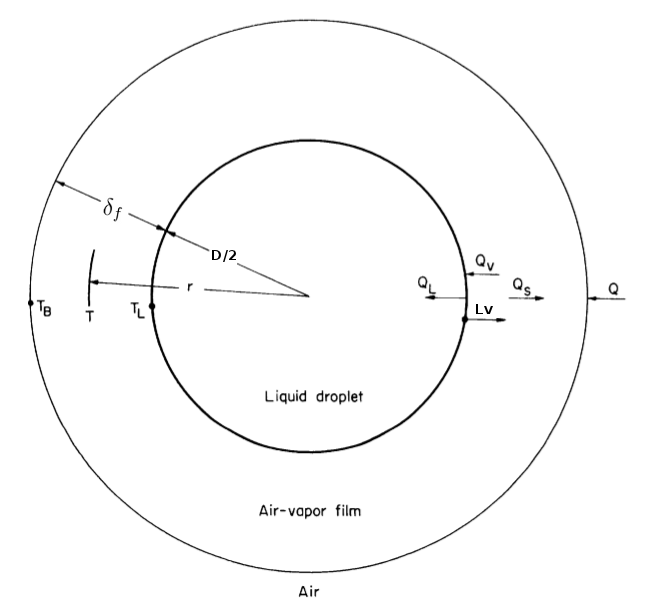
\includegraphics[width=0.8\textwidth]{./figuras/chap2/droplet_heat.png} 
 \caption{Scheme of heat flux from air to droplet, adapted from \cite{naca}.}
 \label{fig: drop_heat}
\end{figure}


\subsubsection{Mass Transfer}

The exposition below follows the already commented simplifications and is commonly denoted as $D^2$-law, see \cite{sirignano}.
Only mass transfer from the droplet to the gas is considered, thus condensation is not allowed.

The steady-state continuity equation for the surrounding gas around the droplet in spherical coordinates is:
\begin{equation}\label{eq: film_mass}
 \frac{d}{d r} \left( \rho u r^2 \right) = 0 \quad \rightarrow \quad \rho u r^2 = cte \, ,
\end{equation}
where $r$ is the radial coordinate and $u$ is the radial velocity.

Using the boundary condition at droplet surface,
\begin{equation}\label{eq: film_species_bc}
 \dot{m}_d = \rho u \left( 4\pi r^2  \right) \, .
\end{equation}
 

The steady-state species equation is:
\begin{equation}\label{eq: film_species}
\frac{d}{d r} \left[ 4\pi r^2 \left( \rho u Y_v -\rho \mathcal{D}_v  \frac{d Y_v}{d r}  \right)\right] = 0\, ,
\end{equation}
where $Y_v$ is the vapor mass fraction and $\mathcal{D}_v$ is the vapor diffusion coefficient. The boundary condition at droplet surface is:
\begin{equation}\label{eq: film_species_bc}
 \left\lbrace 4\pi r^2 \left[ \rho u Y_v -\rho \mathcal{D}_v  \frac{d Y_v}{d r} \right]\right\rbrace  _{r=D/2}  = \dot{m}_d\, . \\
\end{equation}

The integral of \eqref{eq: film_species} using \eqref{eq: film_mass} and \eqref{eq: film_species_bc} may be written as:
\begin{equation}
-\int_{D/2}^{\infty} \frac{\dot{m}_d}{4\pi \rho \mathcal{D}_v}\frac{dr}{r^2} = \int_{Y_{v,s}}^{Y_{v,\infty}} \frac{dY_v}{1-Y_v} \, ,
%- \rho D_v \frac{d Y_v}{d r} = \frac{\dot{m}_d}{4\pi r^2}\left(1-Y_v\right) \, .
\end{equation}
where $Y_{v}$ is the vapor concentration in the air-vapor film. Performing the integration, it becomes:
\begin{equation}
 \frac{dm_d}{dt} = -2\pi D \mathcal{D}_v \rho_v ln \left(
\frac{1-Y_{v,\infty}}{1-Y_{v,s}} \right) \, .
\end{equation}


The vapor mass fraction near the droplet surface ($Y_{v,s}$) is obtained assuming liquid-vapor equilibrium. In this situation, the vapor partial pressure ($p_v$) is given by Clausius-Clapeyron equation:
\begin{equation}
ln \left(\frac{p_v}{p_\infty}\right) = -\frac{L_v W_{v}}{R} \left(\frac{1}{T_d}-\frac{1}{T_b}\right) \, ,
\end{equation}
where $T_b$ is the liquid boiling temperature at pressure $p_{\infty}$ and $L_v$ is the heat of vaporization per unit mass.

Using Raoult's law and the ideal gas state equation, the vapor mass concetration near droplet surface ($Y_{v,s}$) is:
\begin{equation}
Y_{v,s} = \frac{p_v \left(T_d\right)}{p}\frac{W_v}{W} \, .
\end{equation}


The extra mass transfer due to gas motion around the droplet is accounted by the Sherwood number given by the empirical correlation of \cite{ranzmarshall}:
\begin{equation}\label{eq: dropxxxmass}
 \frac{dm_d}{dt} = -2\pi D \mathcal{D}_v \rho_v ln \left(
\frac{1-Y_{v,\infty}}{1-Y_{v,s}} \right) Sh \, ,
\end{equation}
where
\begin{equation}
 Sh = 2.0 +0.6 Re^{1/2} Sc^{1/3} \, .
\end{equation}
As for the Nusselt number, all properties here are computed with the characteristic film temperature ($T^{*}_f$) previously defined.

The droplet evaporation rate ($dm_d/dt$) may then be written as:
\begin{equation}
 \frac{dm_d}{dt}=-\frac{m_d}{\tau_e} \, ,
\end{equation}
where
\begin{equation}\label{eq: tau_e}
 \tau_e = \frac{m_d}{\pi D \mathcal{D} Sh \rho_v ln \left(
\frac{1-Y_{v,\infty}}{1-Y_{v,s}} \right)}
\end{equation}
is the characteristic time scale of droplet evaporation.



% 
% For a droplet temperature above the boiling point, the evaporation occurs at constant temperature and the mass transfer is determined by the rate at which energy is transfered from the gas to the liquid, sustaining the phase change. The equations bellow 
% 
% \begin{equation}
%  \frac{dm_d}{dt}=-\frac{\pi D \kappa Nu}{c_{p,v}} ln \left[ \frac{c_{p,v}}{L_v}
% \left( T- T_d \right) +1 \right]
% \end{equation}
% 
% 
% \begin{equation}
%  \frac{dD}{dt} = -\frac{D}{\tau_{boil}}
% \end{equation}
% 
% \begin{equation}
%  \tau_{boil} = \frac{D^2 \rho_d c_{p,v}}{2 \kappa Nu ln \left[
% \frac{c_{p,v}}{L_v} \left( T- T_d \right) +1 \right]}
% \end{equation}

\subsection{Droplets at Domain Boundaries}

When the droplet crosses the domain boundary, it is simply removed from the computation.

\subsection{Droplet Dispersion}

Although the gas phase velocity has been averaged in \eqref{av: momentum}, the droplet experiences oscillations in its slip velocity if turbulence is present.
This oscillation not only affects the droplet drag, the extra shear on droplet surface might cause deformation and instabilities leading to droplet break-up.
Furthermore, due to changes in the surrounding gas flow, mass and heat transfers are also affected. 

Here, the effects of turbulence on droplet motion are simply accounted for by summing a fluctuation ($\bv{U}''$) to the gas averaged velocity ($\tilde{\bv{U}}$):
\begin{equation}
  \bv{U}_{slip} = \bv{U_d} - \left( \tilde{\bv{U}}+\bv{U}'' \right) \, . \tag{\ref{eq: Urel}}
\end{equation}

For the k-epsilon model, a characteristic magnitude for velocity fluctuation may be defined as the scalar
\begin{equation}
 <U''>= \sqrt{\frac{2}{3} k} \, .
\end{equation}

The magnitude of the velocity fluctuation ($\bv{U}''$) is then sampled from a Gaussian distribution with a variance equal to $<U''>$ and zero mean. Finally, the direction of $\bv{U}''$  is randomly chosen.

The sampling is performed once the time passed from the last sampling is greater than the characteristic time $\tau_{turb}$: the minimum between the eddy lifetime and the time taken to the droplet to cross it, given by the ratio of a turbulent length scale ($l_t = C_{\mu}^{3/4} k^{3/2} / \epsilon $) and the magnitude of the droplet slip velocity:

\begin{equation}
 \tau_{turb} = min \left[ \frac{k}{\epsilon} , \frac{k^{3/2}}{\epsilon} \frac{C_{\mu}^{3/4}}{|\bv{U}_{slip}|}\right] \, .
\end{equation}

Further details are discussed in \cite{kiva} and \cite{baumgarten2006mixture}.


\chapter{The Experiment of Chen, St\aa{}rner and Masri}\label{chap: exp}

Chen, St\aa{}rner and Masri performed at Sydney University a detailed experimental investigation of a turbulent evaporating jet of acetone, see \cite{chen}. Droplet diameter, droplet velocity, droplet number density and liquid volumetric flux were measured using a two-component phase Doppler interferometry (PDI) and acetone vapor mass flux was measured using planar laser-induced fluorescence (PLIF).

The experiment consists of a spray nozzle centered on the exit plane of a wind tunnel with 150mm by 150mm that supplies a co-flowing air stream, see Figure \ref{spray_jet}. 
Inside the nozzle, a pressurized liquid jet is surrounded by a carrier air flow until the nozzle exit. The co-flow has a low turbulence intensity of less than $2\%$, so that the effect on the spray jet turbulence is negligible. The main benefit of this setup is the avoidance of flow recirculation near the nozzle exit, what would be an extra complication for the boundary conditions of a numerical simulation.

Acetone evaporation takes place even before the nozzle exit, cooling both the gas and the droplets. The exit temperature shown in Table \ref{table: experiment} was not measured, but computed from energy conservation based on the measurement of acetone vapor mass flux and  the assumption of thermal equilibrium.

\begin{notation}
Sauter mean diameter - SMD or $D_{32}$ - is an average droplet diameter given by:
\begin{equation}
 SMD= \frac{\sum_{droplets} D^3}{\sum_{droplets} D^2} \, .
\end{equation}
\end{notation}

\begin{table}
\centering
 \begin{tabular}{lc}
\hline
Experiment  Data & \\ \hline
Liquid Phase & Acetone \\
Liquid Flow rate at nozzle exit $(g/min)$  &  $7.0$ \\
Carrier air flow rate $(g/min)$ & $135$ \\
Vapor flux at nozzle exit $(g/min)$ & $5.0$ \\
SMD at nozzle exit $(\mu m)$ & $13.7$ \\
Gas temperature at nozzle exit $(K)$ & $280$ \\ 
Gas jet Reynolds Number $(Re=4 \dot{m}_g/\pi D_{nozzle} \mu_g)$ & $16,300$ \\
\hline
 \end{tabular}
\caption{Basic information about the experiment of Chen, St\aa{}rner and Masri, \cite{chen}.}
\label{table: experiment}
\end{table} 


\begin{figure}[!htb]
 \centering
 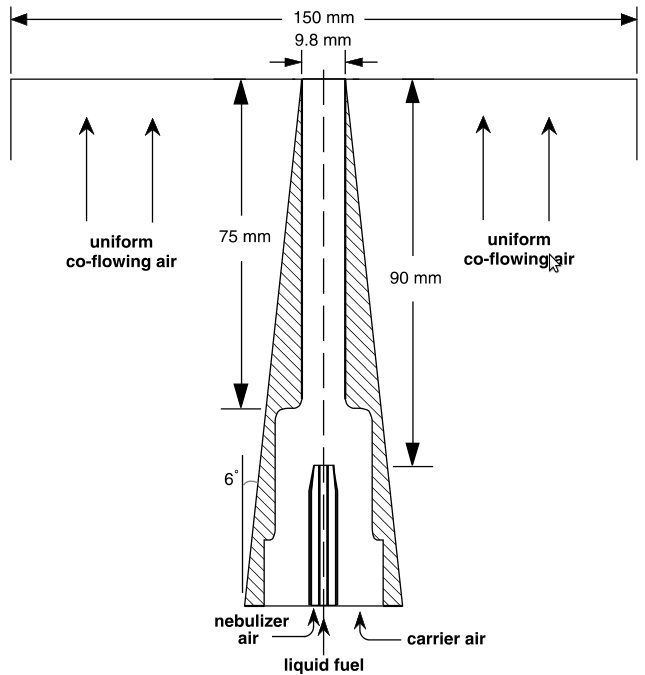
\includegraphics[width=0.4\textheight]{./figuras/chap3/setup.png}
 \caption{Configuration of the spray jet nozzle from \cite{chen}.}
 \label{spray_jet}
\end{figure}

\FloatBarrier
 \section[Boundary Conditions for the Numerical Simulation]{Determining the Boundary Conditions for the Numerical Simulation}

In this section, the boundary conditions for the numerical simulation are obtained from the evailable experimental data. The measurements provide almost complete data for establishing the boundary conditions and few assumptions had to be made.
The list of conditions to be specified for each phase is summarized below.

\subsection{Nozzle}

Below, the boundary conditions at nozzle exit.

\subsubsection{Liquid Phase:}

\begin{description}
  \item[Diameter ($D$):] 
  
The parcel diameter is sampled from a statical distribution built from measurements. \cite{chen} does not provide such measurements at the nozzle exit plane, but only the Sauter mean diameter.  A Lognormal distribution was then specified with $\mu = 10\ \mu m$ and $\sigma=5.5\ \mu m$.

\begin{equation}
 cpf(d; \mu, \sigma) = \frac12 \operatorname{erfc}\!\left[-\frac{\ln D - \mu}{\sigma\sqrt{2}}\right] = \Phi\bigg(\frac{\ln D - \mu}{\sigma}\bigg) \, ,
\end{equation}

\begin{equation}
 pdf(D;\mu,\sigma) = \frac{1}{D \sigma \sqrt{2 \pi}}\, e^{-\frac{(\ln D - \mu)^2}{2\sigma^2}} \, .
\end{equation}

Figure \ref{fig: lognormal} shows the distribution shape. The correspondent Sauter mean diameter is $SMD =14\ \mu m$.
\begin{figure}[!htb]
\centering
  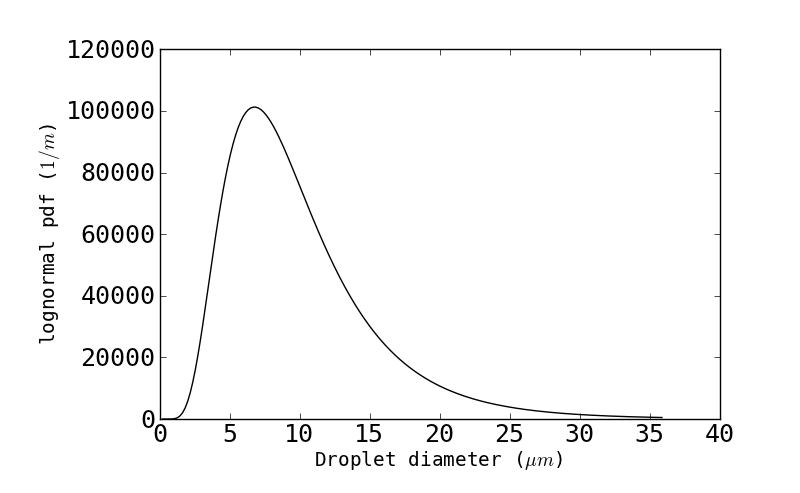
\includegraphics[width=0.75\textwidth]{./figuras/chap3/lognormal.png}
\caption{Lognormal probability density function used for sampling droplet diameter at nozzle exit.}
\label{fig: lognormal}
\end{figure} 
  
\item[Position ($\bv{x}_d$):]
The droplets are inserted in the domain with an aleatory radial coordinate in the interval going from the nozzle axis to the nozzle external radius $(y \in [0, 4.9] \ mm )$, which is sampled for each parcel injection. 
  
  
  \item[Velocity ($\bv{U}_d$):]
  The droplet injection velocity was made dependent only on the injection position according to Figure \ref{fig: bc_dropU}.
  
  \begin{figure}[h]
  \centering
  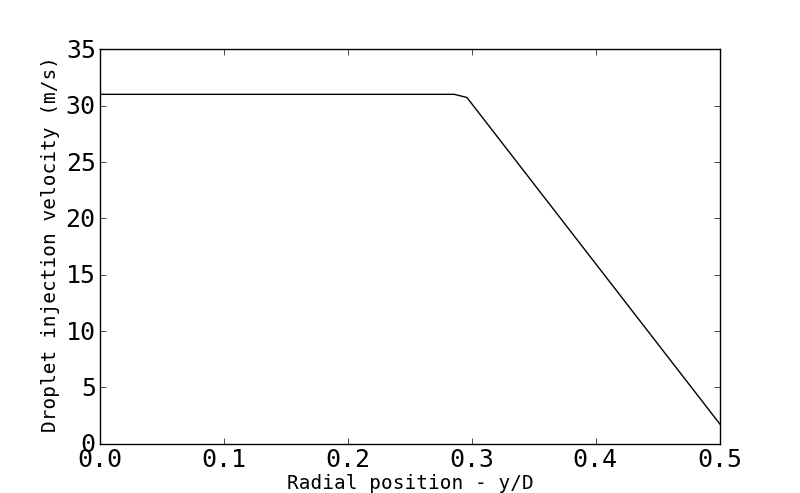
\includegraphics[width=0.65\textwidth]{./figuras/chap3/bc/bc_dropU.png}
  \caption{Droplet injection velocity as a function of its injection position.}
  \label{fig: bc_dropU}
  \end{figure} 
  
  \item[Temperature ($T_d$):] The temperature was determined by assuming thermal equilibrium in the nozzle exit for given mass flow rates of liquid, air and acetone vapor:
  \begin{equation}\label{eq: bc_est_T}
  T_{nozzle}=T_{\infty} - \frac{\dot{m}_{ac} L_{v}}{\dot{m}_g c_{p,g}+\dot{m}_l c_{p,l}} = 280\ K
  \end{equation}
  where $T_{\infty}$ is the ambient temperature and $L_v$ is the latent heat of vaporization of acetone.
  
  The fixed value of $280\ K$ is specified for droplet and gas temperature. 
  
  \item[Mass flow rate ($\dot{m}_d$):] According to the measurements, the liquid mass flow rate is $\dot{m}_d=2\ g/min$.  The parcel injection rate was $5\times10^5\ parcels/s$, yelding about 35,000 parcels in the computational domain.
  \end{description}
  
\subsubsection{Gas Phase:}
  
\begin{description}
  \item[Velocity ($\tilde{\bv{U}}_{nozzle}(\bv{x})$), Turbulent KE ($k_{nozzle}(\bv{x})$) and Dissipation Rate ($\epsilon_{nozzle}(\bv{x})$):] The droplet velocity was obtained from a gas phase only numerical simulation of the nozzle interior with fixed mass flow rate of $\dot{m}_g = 140 g/min$. The turbulence properties in the nozzle inlet was estimated using the following relations from \cite{luppes}:
  \begin{equation}
  k=\frac{3}{2} i^2 \bar{U}_{nozzle}^{2}\, , \quad \epsilon = \frac{c_{\mu}^{3/4} k^{3/2}}{l_m} \, ,
  \end{equation}
  where $\bar{U}_{nozzle}$ is the average velocity inside the nozzle, $i=0.03$ and $l_m = 0.07 D_{nozzle}$.
  The resulting velocity profile was then compared to the mean velocity of the smallest droplets showing good agreement in Figure \ref{fig: bc_gas}.
  
  \item[Temperature ($\tilde{T}_{nozzle}$):] As explained in the liquid phase section, the fixed value of $280\ K$ was used.
  \item[Species Concentration ($\tilde{Y}_{k,nozzle}$):] Given the measured mass flow rates of air ($\dot{m}_{air}$) and acetone vapor ($\dot{m}_{ac}$):
  \begin{equation}
  \begin{split}
  Y_{ac} &= \frac{\dot{m}_{ac}}{\dot{m}_{ac}+\dot{m}_{air}}=0.0357 \, , \\
  Y_{O2} &= 0.233\left( 1- Y_{ac} \right)=0.224 \, , \\
  Y_{N2} &= 1- Y_{ac}-Y_{O2}=0.740 \, .
   \end{split}
  \end{equation}
  \item[Dynamic Pressure ($p_{d,nozzle}$):] A zero gradient condition was used.
\end{description}


\begin{figure}[!htb]
 \centering
\begin{tabular}{cc}
 \subfloat[]{\label{fig: bc_Ux}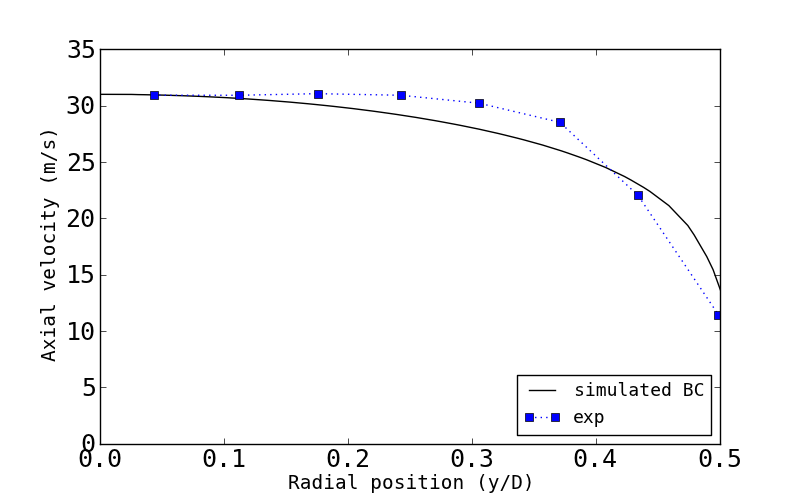
\includegraphics[width=0.5\textwidth]{./figuras/chap3/bc/bc_Ux.png}} &  \subfloat[]{\label{fig: bc_k}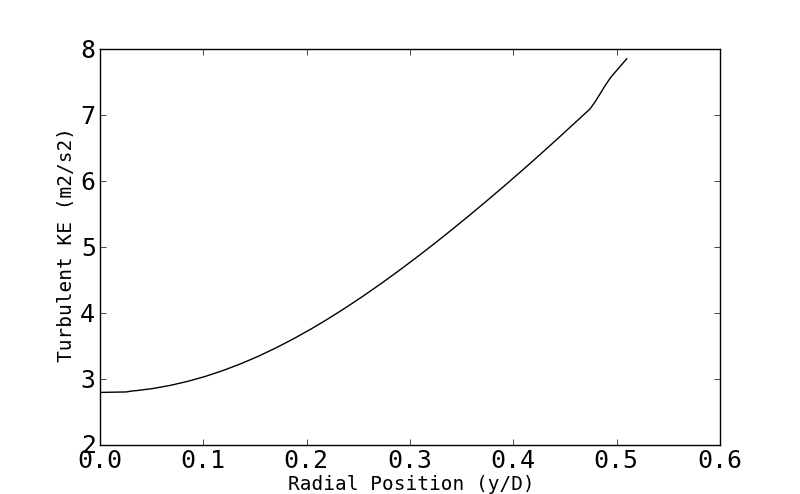
\includegraphics[width=0.5\textwidth]{./figuras/chap3/bc/bc_k.png}} \\
  \subfloat[]{\label{fig: bc_eps}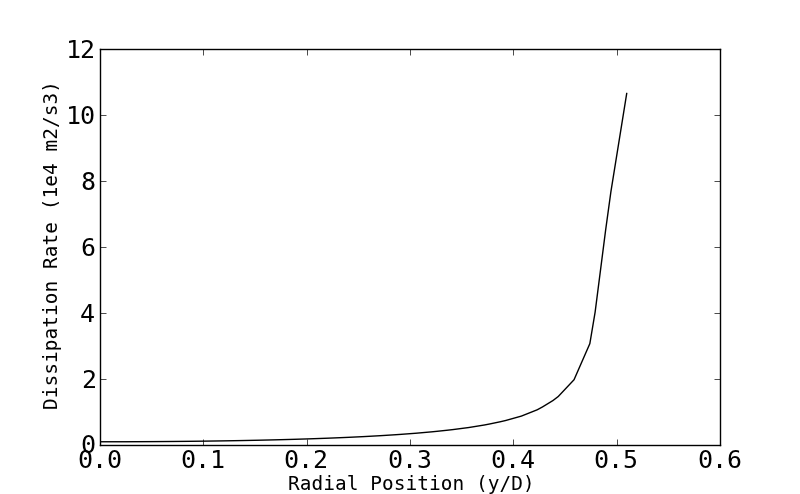
\includegraphics[width=0.5\textwidth]{./figuras/chap3/bc/bc_eps.png}} 
\end{tabular}
 \caption{Radial profiles of the boundary conditions for the gas phase at the nozzle exit plane: mean axial velocity (a), turbulent kinetic energy (b) and its dissipation rate (c).}
 \label{fig: bc_gas}
\end{figure}

\FloatBarrier
\subsection{Coflow}

In the co-flow boundary, only the gas phase is present.

\begin{description}
  \item[Velocity ($\tilde{\bv{U}}_{co-flow}$), Turbulent KE ($k_{co-flow}$) and Dissipation Rate ($\epsilon_{co-flow}$):] A fixed value for velocity was used with the same relations for turbulence properties from \cite{luppes}:
  \begin{equation}
  \begin{split}
  &\tilde{U}_{co-flow} =3\ m/s\, ,\\
   & k =\frac{3}{2} i^2 \bar{U}_{nozzle}^{2}= 0.0054\ J/kg \, , \\
   &\epsilon = \frac{c_{\mu}^{3/4} k^{3/2}}{l_m}=0.0124\ J/kg/s \, ,
  \end{split}
  \end{equation}
  where $\bar{U}_{nozzle}$ is the average velocity in the co-flow region, $i=0.02$ and $l_m = 0.07 D_{co-flow}$.
  
  \item[Temperature ($\tilde{T}_{co-flow}$):] The fixed value of $298\ K$ was used, the ambient temperature.
  \item[Species Concentration ($\tilde{Y}_{k,co-flow}$):] Given the measured mass flow rates of air ($\dot{m}_{air}$) and acetone vapor ($\dot{m}_{ac}$):
  \begin{equation}
  Y_{ac} = 0 \, , \quad Y_{O2} = 0.233 , \quad Y_{N2} = 0.767 \, .
  \end{equation}
  \item[Dynamic Pressure ($p_{d,co-flow}$):] A zero gradient condition was used.
\end{description}

\subsection{Far-field}

Ambient pressure ($p_{\infty}=1\times 10^5\ Pa$) is set for dynamic pressure. Zero gradient is set for the remaining quantities.

\section{Species Equations}

It is only considered the presence of two species: acetone vapor and air. Equation \eqref{av: species1} for the mean mass concentration of acetone vapor ($\tilde{Y}_{ac}$) is then
\begin{equation}
 \frac{\partial \bar{\rho} \tilde{Y}_{ac} }{\partial t} + \nabla
\cdot\left(\bar{\rho} \tilde{\bv{U}} \tilde{Y}_{ac} \right) = \nabla \cdot \left[ \bar{\rho} \left( \nu + \nu_T \right)
\nabla \tilde{Y}_{ac} \right] +\bar{S}_{Yac} \, ,
\end{equation}
The acetone vapor is the scarce species relative to air,
\begin{equation}
\tilde{Y}_{air} = \tilde{Y}_{O2} + \tilde{Y}_{N2}= 1- \tilde{Y}_{ac} \, .
\end{equation}


\chapter{Numerical Solution and Computational Details}\label{chap: numerical}
\section{Numerical Solution of Equations}

\subsection{The OpenFOAM Code}

The numerical solution of the equations presented in Chapter \ref{chap: equations} was obtained using the OpenFOAM code. Details of OpenFOAM formulation are explained in \cite{jasak} and \cite{weller}.  From all the set of available solvers and libraries in OpenFOAM, the dieselFOAM solver and dieselSpray class were the major pieces of code used in this work. To my knowledge, both were written by Niklas Nordin, \cite{nordin}.

The dieselSpray class handles the modeling of lagrangian particles and their submodels. Minor modifications were made in order to have more flexibility in boundary conditions and to adapt them to the experimental conditions.

The dieselFOAM solver couples the modeling of the lagrangian particles and the gas flow solution. The spray sources are explicitly treated and the coupling among variables is solved with PISO algorithm, see \cite{jasak} and \cite{ferziger}.

Minor modifications were added to the solution of low Mach number equations instead of the fully compressible formulation.
They are briefly explained here, but the understanding requires from the reader some familiarity with OpenFOAM programming.

The thermodynamic pressure retained its original name \verb|p| and is the pressure used in the state equation:
\begin{verbatim}
<createFields.H>
volScalarField& p = thermo.p();                               
\end{verbatim} 
and in the lagrangian models:
\begin{verbatim}
<createSpray.H>
spray dieselSpray
(
    U,
    rho,
    p,
    T,
    composition,
    gasProperties,
    thermo,
    g
);\end{verbatim} 

A new scalar field was assigned to the dynamic pressure, \verb|volumeScalarField pd|:
\begin{verbatim}
<createFields.H>
 volScalarField pd
(
    IOobject
    (
        "pd",
        runTime.timeName(),
        mesh,
        IOobject::MUST_READ,
        IOobject::AUTO_WRITE
    ),
    mesh
);
\end{verbatim} 

The momentum equation was modified to be computed using the gradient of \verb|pd| instead of \verb|p| in the momentum predictor:
\begin{verbatim}
<UEqn.H>
     fvVectorMatrix UEqn
    (
        fvm::ddt(rho, U)
      + fvm::div(phi, U)
      + turbulence->divDevRhoReff(U)
     ==
        rho*g
      + dieselSpray.momentumSource()
    );

    if (momentumPredictor)
    {
        solve(UEqn == -fvc::grad(pd));
    }
\end{verbatim} 

Finally, the the pressure equation is now a Poisson equation for the dynamic pressure and it uses the thermodynamic presure for computing the density.
\begin{verbatim}
<pEqn.H>

  fvScalarMatrix pdEqn
  (
      fvc::ddt(psi,p)
      + fvc::div(phi)
      - fvm::laplacian(rho*rUA, pd)
      ==
      Sevap
  );
\end{verbatim} 
where \verb|psi| or $\Psi$ is the isothermal compressibility. For an ideal gas:
\begin{equation}
 \rho=p\Psi=\frac{p}{RWT} \, .
\end{equation}

In this work, the time-dependence of the thermodynamic pressure is neglected and the therm \verb|fvc::ddt(psi,p)| vanishes.

\section{Aspects of the Numerical Solution}
The calculations deviate from experiments due to three groups of errors as stated in \cite{jasak} and briefly explained here:
 
\begin{description}
 \item[Modeling Errors:] the difference of the real flow and the exact solution of the mathematical model.
 \item[Discretization Errors:] the difference between the exact solution of the mathematical model and the exact solution of the discretized equations on the discretized domain (the numerical grid).
 \item[Iteration Convergence Errors:] the difference between the approximate and the exact solution of the discretized equations in the discretized domain. The approximate solution is obtained by iterative methods that reduce the convergence error up to a certain level known as the solver tolerance. 
 \end{description}
 
 The modeling errors were already discussed as the governing equations were presented in Chapter \ref{chap: equations}. The discretization of equations is treated in next section. The criterion for iteration convergence was set to $10^{-7}$ for the pressure equation and $10^{-6}$ for the remaining variables. The residual of equations were monitored during execution to ensure the validity of the solution.
 
The equations were solved in segregated linear systems using conjugate gradient algorithms. The solution did not present convergence difficulties as the convergence tolerances were satisfied in few iterations.

\subsection{Discretization of the Governing Equations}
The general transport equation for a scalar intensive property $\phi$ is:
\begin{equation}
 \underbrace{\frac{\partial \rho \phi}{\partial t}}_{\text{temporal derivative}} + \underbrace{\nabla \cdot \left(\rho \bv{U} \phi \right)}_{\text{advection}} - \underbrace{\nabla \cdot \left( \rho \Gamma \nabla \phi \right)}_{\text{diffusion}} = \underbrace{S\left(\phi\right)}_{\text{source}}
\end{equation}


Each term was discretized using the following schemes:
\begin{itemize}
 \item Temporal derivative: Euler implicit method;
 \item Advection term: Gauss theorem is applied to transform the divergence in surface integrals and the upwind scheme is used to interpolate cell centered values to cell faces;
 \item Diffusion term: Gauss theorem with linear interpolation from cell center to faces. Central difference is used for the gradient;
 \item Sources: all sprays sources are explicitly handled. The spray is evolved from time step "n" to "n+1" using the gas phase properties at time step "n", and all source terms are computed. The gas is then evolved to time step "n+1".
\end{itemize}

\subsection{Domain Discretization (The Numerical Grid)}

Two axisymmetric (2D) orthogonal mesh grids were built: a fine and a coarse grid. OpenFOAM uses the collocated grid arrangement. The fine grid was composed of $14,800$ cells ($74$ cells in the radial direction and $200$ in the axial direction) and the coarse grid was composed of $5,460$ cells ($42$ in the radial direction and $130$ in the axial direction). The geometries are shown in Figure \ref{fig: meshes}.

\begin{figure}[!htb]
 \centering
 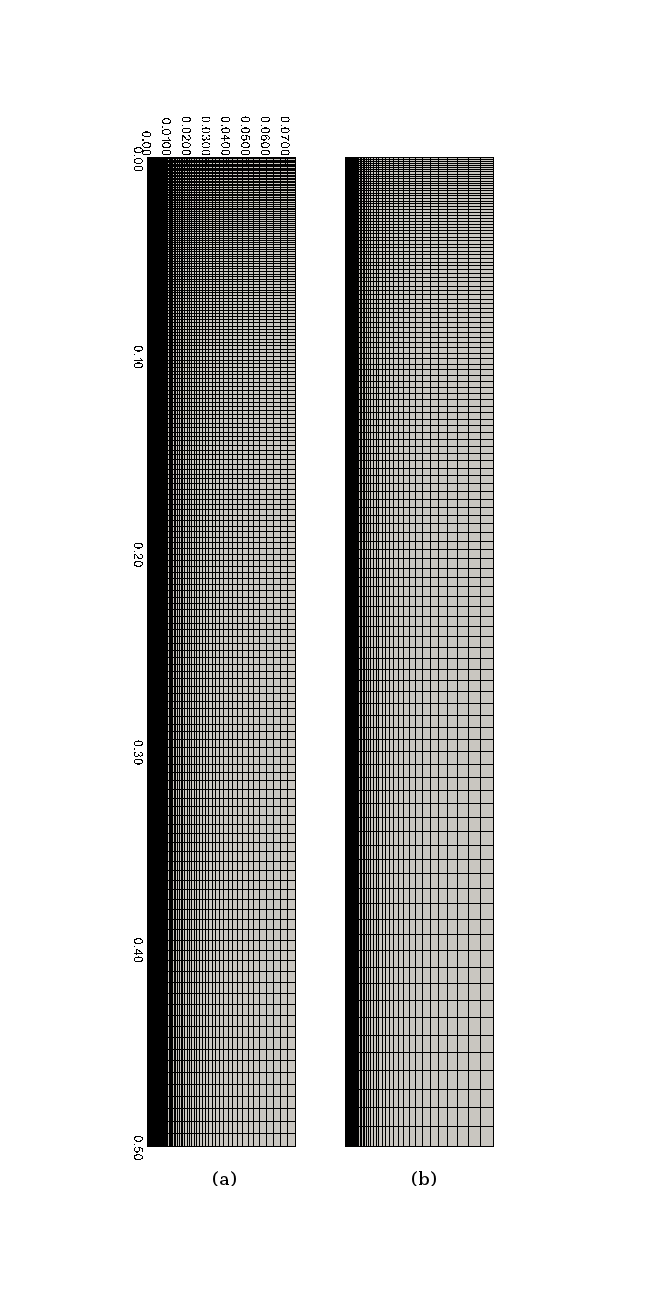
\includegraphics[height=0.9\textheight]{./figuras/chap4/grid.png}
 \caption{Planar view of the fine (a) and the coarse grid (b).}
\label{fig: meshes}
\end{figure}

Solutions for both grids were obtained for a gas phase only flow using the same boundary conditions described in Chapter \ref{chap: exp}, hence the same Reynolds number, and the same discretization schemes for the equations and the same convergence tolerances previously mentioned. 

Figure \ref{fig: grid_test} shows on the left the comparison of radial profiles of mean axial velocity ($\tilde{U}_x$) for the axial coordinates: $x/D=5$, $x/D=15$ and $x/D=25$. In the same Figure, but on the right, it is shown radial profiles of the turbulent kinetic energy ($k$) for the same axial coordinates. In despite of some differences, the coarse grid solution was considered enough accurate and it was used for the results presented in Chapter \ref{chap: results}.

\begin{figure}[h]
 \centering
\begin{tabular}{cc}
 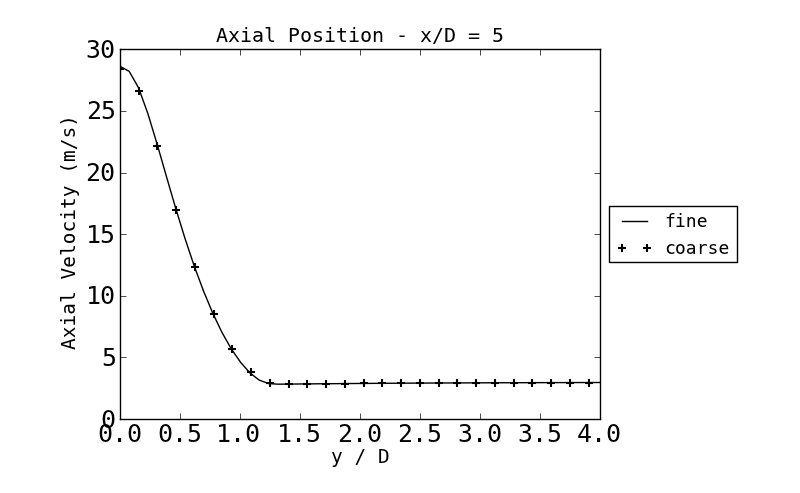
\includegraphics[width=0.5\textwidth]{./figuras/chap4/coarse_fine/grid_0_U.png} & 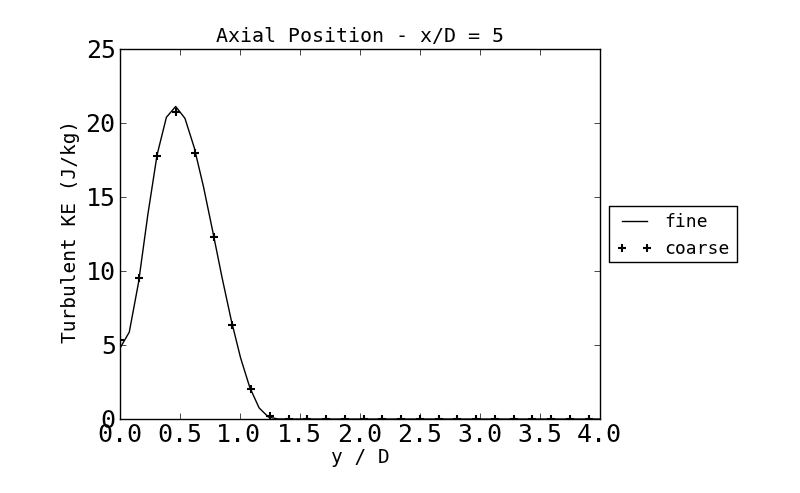
\includegraphics[width=0.5\textwidth]{./figuras/chap4/coarse_fine/grid_0_k.png} \\
(a) & (b) \\
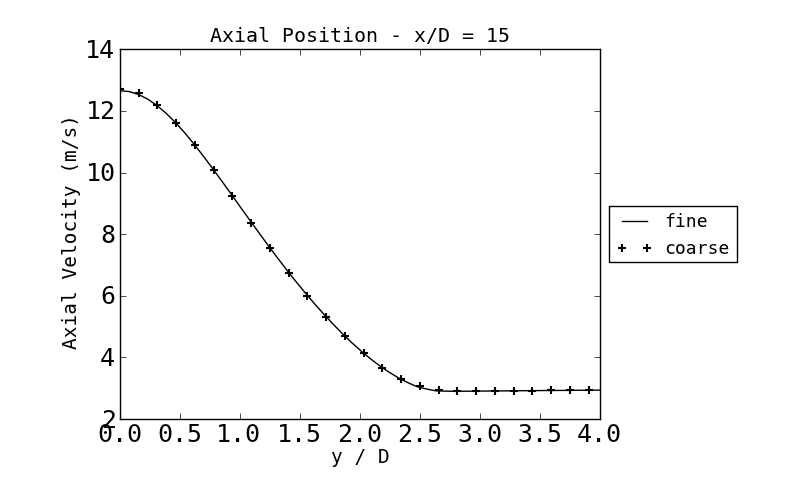
\includegraphics[width=0.5\textwidth]{./figuras/chap4/coarse_fine/grid_2_U.png} & 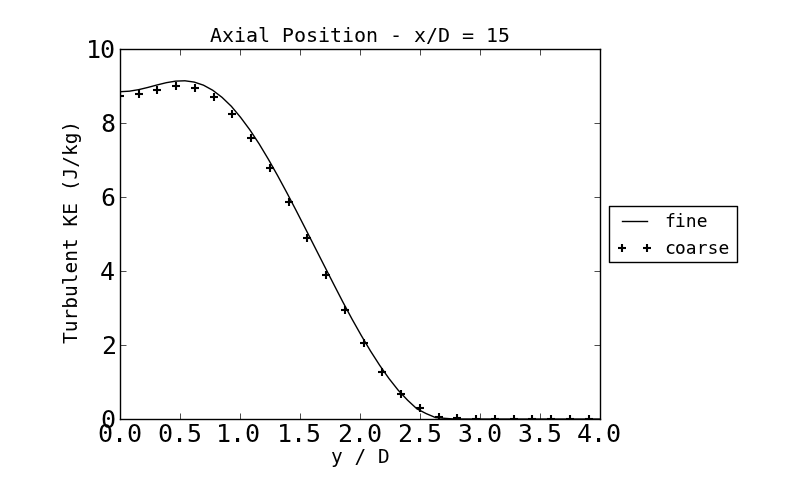
\includegraphics[width=0.5\textwidth]{./figuras/chap4/coarse_fine/grid_2_k.png} \\
(c) & (d) \\
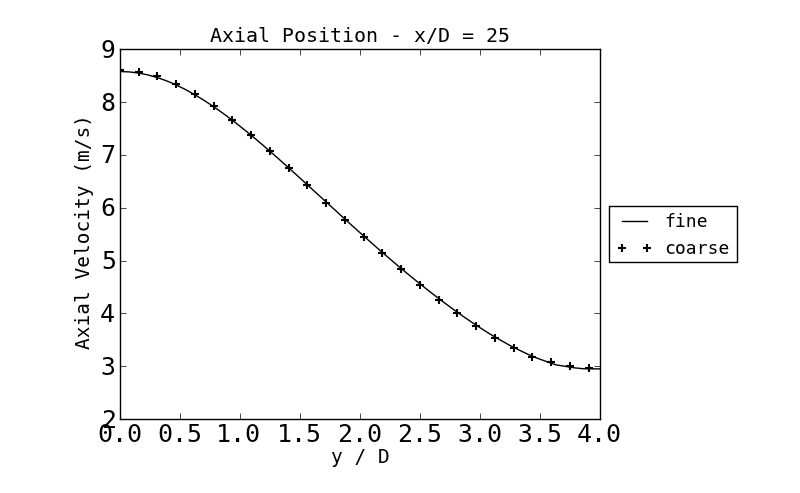
\includegraphics[width=0.5\textwidth]{./figuras/chap4/coarse_fine/grid_4_U.png} &   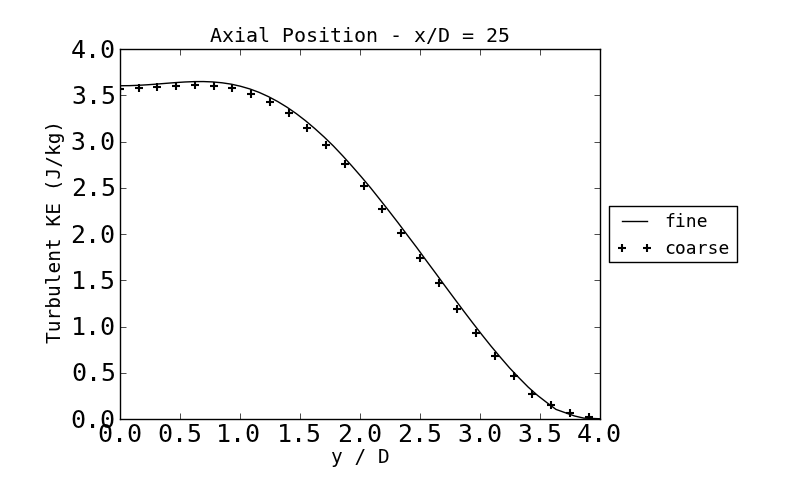
\includegraphics[width=0.5\textwidth]{./figuras/chap4/coarse_fine/grid_4_k.png} \\
(e) & (f)
\end{tabular}
 \caption{Comparison of radial profiles obtained for the fine and the coarse meshes for a pure gaseous jet. Mean axial velocity ($\tilde{U}_x$) on the left for axial coordinates: $x/D=5$ in (a), $x/D=15$ in (c) and $x/D=25$ in (e); and turbulent kinetic energy ($k$) on the right: $x/D=5$ in (b), $x/D=15$ in (d) and $x/D=25$ in (f).}
 \label{fig: grid_test}
\end{figure}

It is not clear how mesh refinements will necessarily improve computations for the lagrangian description of droplets. This happens because it is made the assumption that the liquid volume fraction in the computational cell is negligible. If the mesh is refined further and further, this might become untrue. For the present work, the liquid volumetric fraction in the cells near the nozzle is about $10^{-3}$ for the fine mesh and about $10^{-5}$ for the coarse mesh.

Another problem with mesh refinement using the lagrangian-eulerian approach is the differences obtained in interpolating gas properties to parcel positions from one grid to another. This problem has been discussed in \cite{nordin} and \cite{baumgarten2006mixture}. 

So far, the recommendation for the mesh dependency is to refine the cells until certain accuracy for the continuous phase is satisfied and not until the eventual limitation of computational cost, what could violate the assumption of a low liquid volume fraction.

% DROPLET TRACKING
% PISO ALGORITHM


\chapter{Results and Discussions}\label{chap: results}

In this chapter, it is presented results and discussions on numerical simulation of the experiment of \cite{chen} using the methodology introduced in the preceding chapters. The first section shows results of spread rate and self-similar profiles of the gas phase turbulent jet. The second section shows results of droplet and gas velocities and droplet dispersion. The third section presents liquid mass flow rates, vapor mass fluxes and droplet Sauter mean diameter.

\section{The Turbulent Round jet}

Consider the following definitions for the turbulent round jet:
\begin{description}
 \item[Jet half-radius ($y_{1/2}(x)$):] the radial coordinate for which the mean axial velocity is half of the mean axial velocity at the centerline for some axial coordinate $x$:
\begin{equation}
\tilde{U}_x (y=y_{1/2}) = \frac{1}{2}\tilde{U}_x(y=0) \, .
\end{equation}
\item[Dimensionless radial coordinate ($\hat{y}(x,y)$):]
\begin{equation}
 \hat{y} = \frac{y}{y_{1/2}} \, .
\end{equation}

\item[Dimensionless Mean Axial Velocity ($\hat{U}$):]
\begin{equation}
 \hat{U} = \frac{\tilde{U}_x-\tilde{U}_{\text{co-flow}}}{\tilde{U}_x (y=0)-\tilde{U}_{\text{co-flow}}} \, ,
\end{equation}
where $\tilde{U}_{\text{co-flow}}$ is the mean axial velocity of the co-flow stream specified in the boundary condition.

\item[Dimensionless Turbulent Kinetic Energy $\hat{k}$:]
\begin{equation}
 \hat{k}=\frac{k}{(\tilde{U}_x (y=0)-\tilde{U}_{\text{co-flow}})^2} \, .
\end{equation}

\item[Dimensionless Turbulent Viscosity ($\hat{\nu}_T$):]
\begin{equation}
\hat{\nu}_T = \frac{\mu}{\bar{\rho}\tilde{U}_x(y=0) y_{1/2}} \, .
\end{equation}

\item[Jet Spread Rate ($S$):]
\begin{equation}
S = \frac{d y_{1/2} (x)}{dx} \, .
\end{equation}
\end{description}

An empirical observation of a gas turbulent round jet is that the profiles of $\hat{U}$, $\hat{k}$ and $\hat{\nu}_T$ as function of $\hat{y}$ becomes self-similar (i.e. independent of the axial coordinate) from some distance to the nozzle exit.
Furthermore, there is a linear relation between the half-radius ($y_{1/2}$) and the axial coordinate, that is, the jet sprad rate is constant.

\cite{chen} has experimentally shown that self-similarity also occurred for $\hat{U}$ in the presence of the spray jet for $x/D \ge 10$. For arriving at this conclusion, it assumed the velocity measured for the smaller droplets ($D<3\mu m$) as being the gas velocity. 

The group of Figures \ref{fig: selfsimilar_profile} shows the same investigation for the gas velocity field obtained in the numerical simulation. The Figure \ref{ssA} shows the profiles of $\hat{U}$ for several axial coordinates. Differently than the experiment, the self-similarity only occurs for $x/D \ge 15$ (and not for $x/D \ge 10$). This suggests that the transition from the jet developing region to the turbulent region is retarded in the simulation.

\begin{notation}
$<f''>$ or $<f'>$ denotes the root mean square of the fluctuation $f''$ (for a Favre average) or $f'$ (for a time average).
\end{notation}

Figures \ref{ssB} and \ref{ssC} show that the evolution to self-similar profiles is slower for the turbulent quantities $\hat{k}$ and $\hat{\nu}_T$ and one may not say that the self-similarity was achieved inside the domain. \cite{chen} has shown that for $x/D \le 25$ it was also not achieved in the experiment for the root mean square of the axial velocity fluctuation ($<U''_x>$). 

One observation concerning the turbulent viscosity ($\hat{\nu}_T$) is that the centerline value seems to evolve to a value of $\hat{\nu}_T = 0.047$, higher than values found in the literature for the turbulent round jet. \cite{pope2000turbulent} reports a self-similar turbulent viscosity at centerline of $\hat{\nu}_T = 0.029$.


\begin{figure}[!htb]
 \centering
\begin{tabular}{c}
 \subfloat[]{\label{ssA}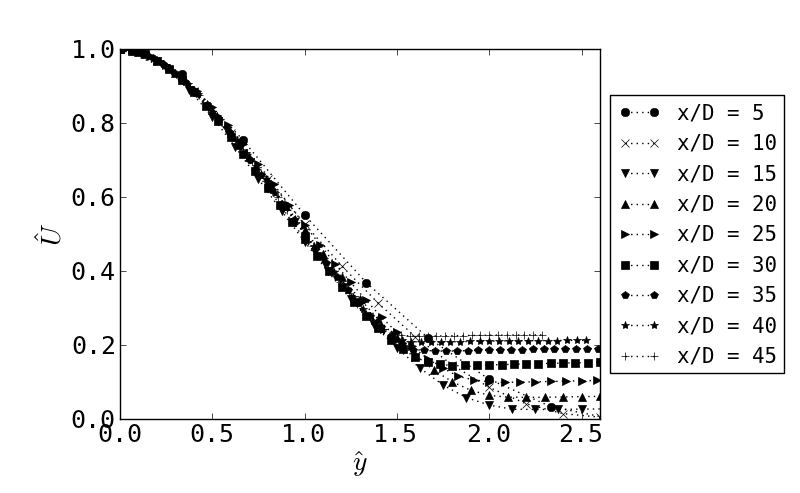
\includegraphics[width=0.65\textwidth]{./figuras/chap5/selfsimilar/selfsimilar_U.png}} \\
 \subfloat[]{\label{ssB}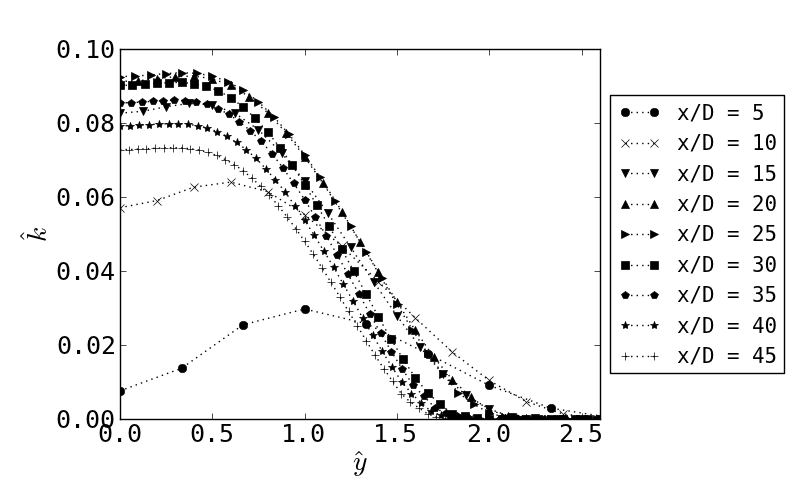
\includegraphics[width=0.65\textwidth]{./figuras/chap5/selfsimilar/selfsimilar_k.png}} \\
 \subfloat[]{\label{ssC}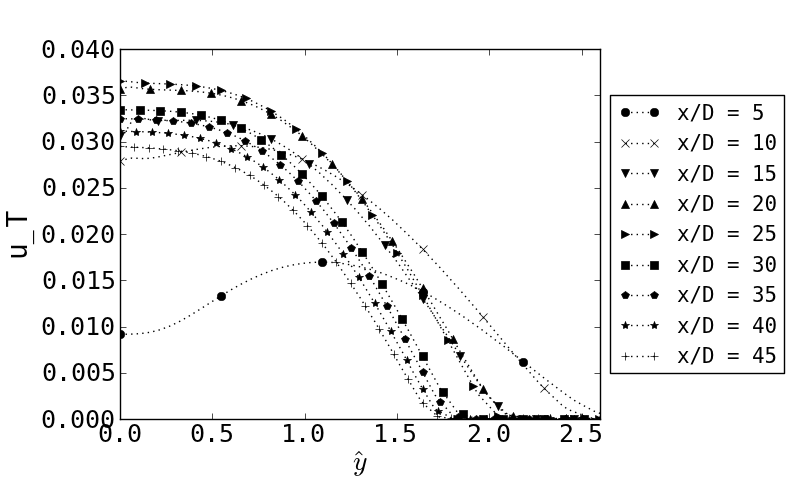
\includegraphics[width=0.65\textwidth]{./figuras/chap5/selfsimilar/selfsimilar_nut.png}} \\
\end{tabular}
 \caption{Numerical results showing the evolution to self-similar profiles of the following gas phase properties: (a) dimensionless mean axial velocity - $\hat{U}_x$, (b) dimensionless turbulent kinetic energy - $\hat{k}$ - and (c) dimensionless turbulent viscosity - $\hat{\nu}_t$. The different curves show the profiles for the corresponding axial coordinate indicated in the legend.}
\label{fig: selfsimilar_profile}
\end{figure}

The jet spread rate measures the spread of the axial velocity in the radial direction. A value about $S=0.095$ is found on the literature for the pure gas flow \cite{pope2000turbulent}, and it is independent of Reynolds number. For the spray jet, however, \cite{chen} has reported $S=0.066$. In the simulation, it was found a higher value of $S=0.071$, a difference of $23\%$. 

The Figure \ref{fig: ssS} shows the indeed different half-radius values found in the simulation and the experiment for the same axial coordinates, and Figure \ref{fig: ssP} compares the self-similar profiles of $\hat{U}_x$ from the simulation and the experiment.

The overestimation of the round jet spread rate with the default coefficients of k-epsilon turbulence model has been reported previously by different authors. \cite{luppes} has discussed four alternatives to the correction. The modifications consist not only in changing the model coefficients, but also tunning of boundary conditions. 

No correction was used in this work because the exact modifications are not known in advance. The effect of this discrepancy on the droplet velocities is discussed in the next section. 

\begin{figure}[!htb]
 \centering
\begin{tabular}{cc}
 \subfloat[]{\label{fig: ssS}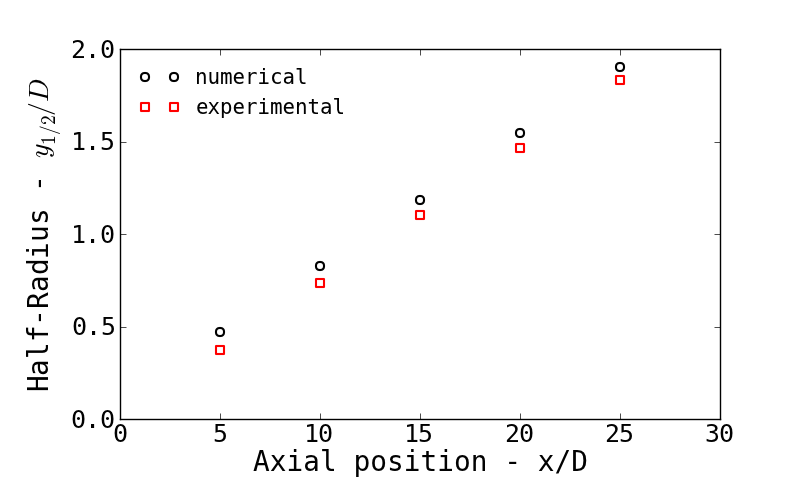
\includegraphics[width=0.5\textwidth]{./figuras/chap5/selfsimilar/selfsimilar_spread.png}} & \subfloat[]{\label{fig: ssP}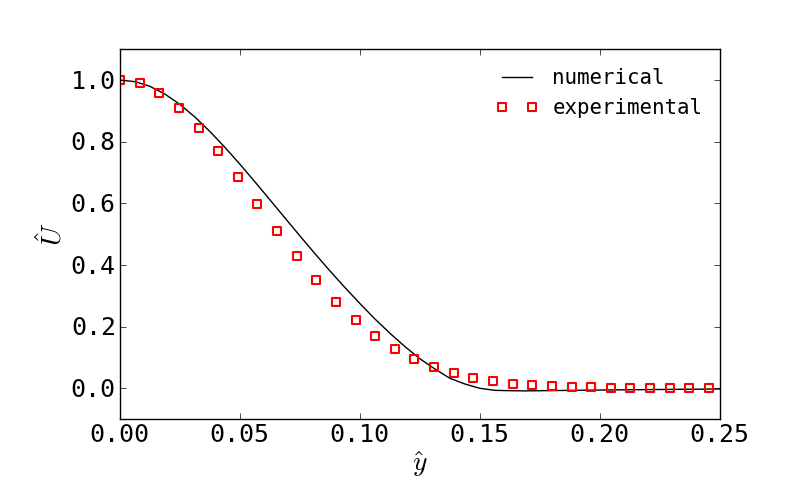
\includegraphics[width=0.5\textwidth]{./figuras/chap5/selfsimilar/selfsimilar_num_exp.png}}
\end{tabular}
 \caption{(a) Half-radius as a function of the axial coordinate in the experiment and in the simulation.  (b) Self-similar radial profile of the numerical and the experimental dimensionless axial velocity - $\hat{U}_x$. The measurements were obtained from \cite{chen}.}
\label{fig: selfsimilar_spread}
\end{figure}

\FloatBarrier
\section{Gas and Droplet Velocities and Droplet Dispersion}

\cite{chen} has presented velocity measurements for droplets of four diameter classes in the spray jet: $D< 5\mu m$, $10\mu m <D<20\mu m$, $20 \mu m < D < 30 \mu m$ and $30 \mu m < D < 40 \mu m$. The importance of separating the data in droplet size classes is that the drag force is dependent on its size. 

Figure \ref{fig: drop_drag} shows the time response to drag force as modeled in Equation \eqref{eq: drop_dudt} for droplets with diameter ranging from $10$ to $40\mu m$ and initial velocity of $10\ m/s$. The time for the droplet with diameter of $40\ \mu m$ comes to rest is nearly $10$ times greater than the required for the droplet with $10\ \mu m$.

\begin{figure}
 \centering
\begin{tabular}{c}
 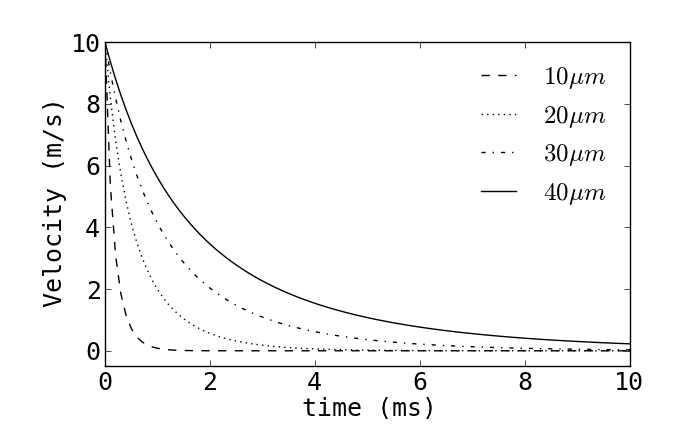
\includegraphics[width=0.65\textwidth]{./figuras/chap5/drag/drop_drag.png}
\end{tabular}
 \caption{Solution of droplet drag model of Equation \eqref{eq: drop_dudt}. Droplet velocity as a function of time for an initial velocity of $10\ m/s$ in stagnant air at standard conditions and for droplet diameters of $10$, $20$, $30$ and $40 \mu m$. }
 \label{fig: drop_drag}
\end{figure}

% The calculation accuracy of the droplet dispersion is mainly dependent on how much of gas turbulence is resolved and the droplets Stoke number. Higher Stokes numbers ($St \ge 10$) allow less resolution of flow turbulence because droplet is more likely to follow the mean velocity field. 

This fast response of smaller droplets provides a good estimative of the gas velocity. \cite{chen} has measured the velocity of droplets with $D< 5\ \mu m$ that here will be assumed to represent also the experimental gas velocity. The consequences of the larger spread rate mentioned before may then be evaluated directly in the radial profile of the mean axial velocity.

Figure \ref{fig: Ux_gas} shows in red squares the measured radial profiles of the mean axial velocity for the gas phase ($\tilde{U}_x$) in the axial coordinates of: $x/D=5$, $10$, $15$, $20$ and $25$. The radial profile obtained in the simulation is also shown in a solid black line. It is evident that the underprediction of the gas velocity in the simulation becomes higher in the downstream direction. In the axial coordinate of $x/D=25$, the centerline value in the simulation is about $20\%$ below the experimental value.

\begin{figure}[!htb]
 \centering
\begin{tabular}{cc}
 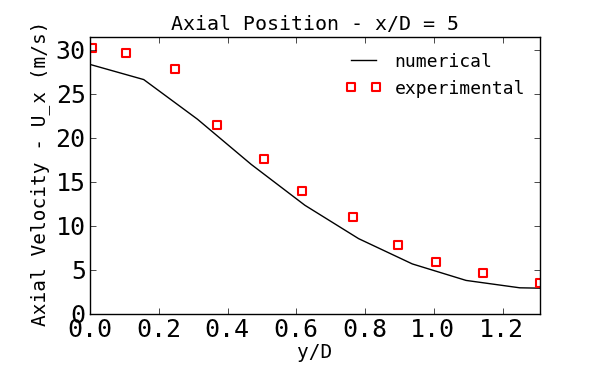
\includegraphics[width=0.5\textwidth]{./figuras/chap5/Ux/Ux_gas/Ux_gas5.png} & 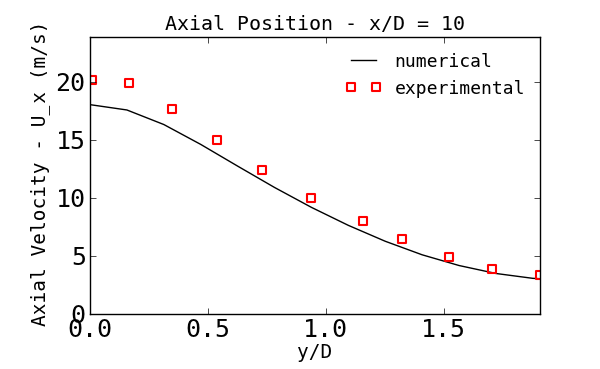
\includegraphics[width=0.5\textwidth]{./figuras/chap5/Ux/Ux_gas/Ux_gas10.png} \\
(a) & (b) \\
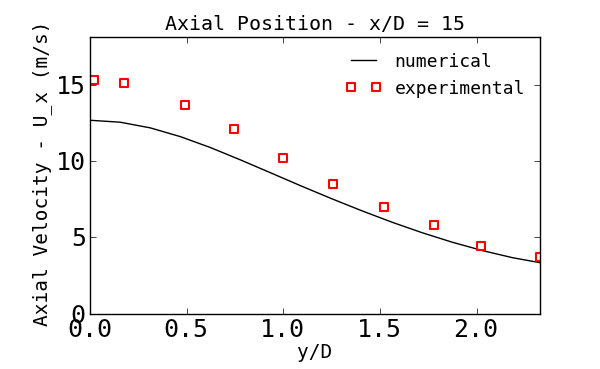
\includegraphics[width=0.5\textwidth]{./figuras/chap5/Ux/Ux_gas/Ux_gas15.png} & 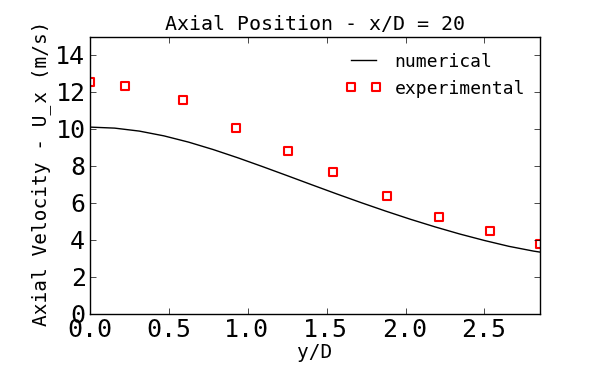
\includegraphics[width=0.5\textwidth]{./figuras/chap5/Ux/Ux_gas/Ux_gas20.png} \\
(c) & (d) \\
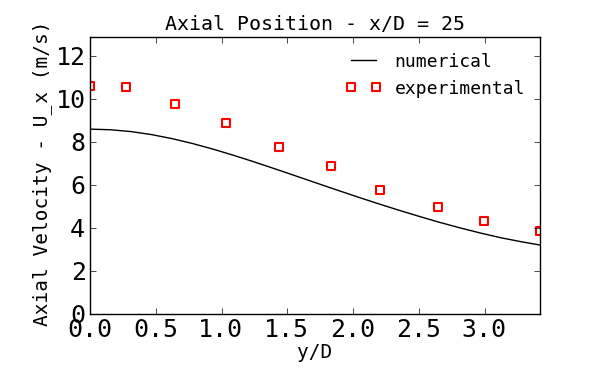
\includegraphics[width=0.5\textwidth]{./figuras/chap5/Ux/Ux_gas/Ux_gas25.png} &   \\
(e) & \\
\end{tabular}
 \caption{Measured and computed radial profiles of the mean axial velocity of the gas phase ($\tilde{U}_x$). Each figure shows the profile in a different axial location: $x/D=5$ in (a), $x/D=10$ in (b), $x/D=15$ in (c), $x/D=20$ in (d) and $x/D=25$ in (e). The measurements were obtained from \cite{chen}.}
 \label{fig: Ux_gas}
\end{figure}

It may be questioned whether the flux of gas momentum in the nozzle exit were correct because the gas exiting temperature was estimated from an assumption of thermal equilibrium with the liquid phase, as explained in Equation \eqref{eq: bc_est_T} in Chapter \ref{chap: exp}. If temperature were lower than in the experiment, then the density and the momentum flux would also be lower.

However, that was not the case. Velocity agreement was good, see Figure \ref{fig: bc_Ux}, and nozzle mass flow rate matches measurements within $1.5\%$. This led to the conclusion that the momentum flux was correctly specified in the nozzle exit and that the discrepancies in velocity were due only to the turbulence modeling.

In fact, \cite{luppes} has reported an error of the same percentual magnitude using the k-epsilon model with the default coefficients. This result is reproduced in Figure \ref{fig: luppes}. The simulation with default k-epsilon coefficients is represented as the curve \textit{simulation 1}. The others curves are results obtained by tunning the model parameters and the boundary conditions.

\begin{figure}[!htb]
 \centering
\begin{tabular}{c}
 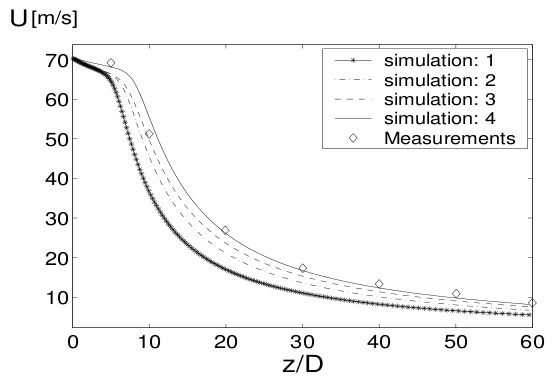
\includegraphics[width=0.6\textwidth]{./figuras/chap5/refs/luppes_vel.png} 
\end{tabular}
 \caption{The comparison of four simulations of a turbulent air jet (Re = 37,600) with measurements. The centerline axial velocity is shown. In each plot the axial distance is normalized by the nozzle diameter. Simulation 1:
standard k-epsilon model. Simulation 2: $c_{\mu} =0.06$. Simulation 3: $c_{\mu}=0.06$, $c_{\epsilon, 2} =1.87$. Simulation 4: $c_{\mu}=0.09$, $c_{\epsilon, 2}=1.87$, n =10. Figure reproduced from \cite{luppes}.}
 \label{fig: luppes}
\end{figure}

 \cite{chen} has also reported the root mean square of axial and radial velocities, respectively $<U''_x>$ and $<U''_y>$. Again, the values for the smaller droplets ($D< 5\ \mu m$) are being used to represent the gas velocity. The same quantities are not provided in the simulation for direct comparison. The turbulence model only solves for the turbulent kinetic energy and its dissipation rate. A characteristic velocity, however, may be defined as $<U''>=\sqrt{2/3 k}$. This quantity is shown in Figure \ref{fig: UUx} with $<U''_x>$ and $<U''_y>$. Again, it is shown radial profiles for different axial coordinates.

Three observations are readily made:  
\begin{itemize}
  \item The radial profile of $<U''_x>$ is similar to that of $<U''_y>$;
  \item The characteristic velocity defined for the k-epsilon model ($<U''>$) agrees well with $<U''_x>$ and $<U''_y>$;
 \item $<U''>$ declines faster than $<U''_x>$ and $<U''_y>$ as the axial coordinate increases.
\end{itemize}

The first observation indicates that the turbulent jet differs from the self-similar profiles found in the literature \cite{pope2000turbulent}, where $<U''_x>$ is about twice as big as $<U''_y>$ in the centerline. It remains the question whether this occurs because the jet is not fully developed or because of some spray influence.

The second observation suggests that the k-epsilon model is appropriate to describe the round jet turbulence, providing an appropriate characteristic velocity. The third observation, however, indicates that the turbulent dissipation is overpredicted.

\begin{figure}[!htb]
 \centering
\begin{tabular}{cc}
 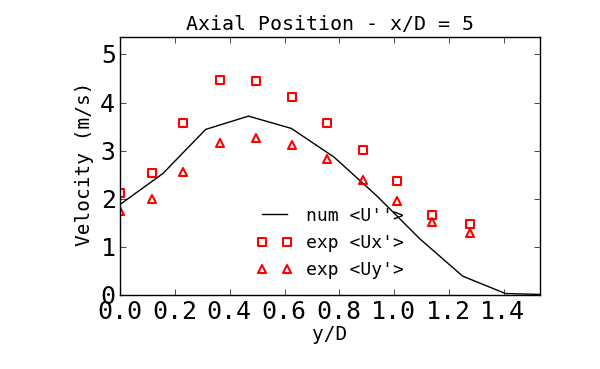
\includegraphics[width=0.5\textwidth]{./figuras/chap5/UU/UUx5.png} & 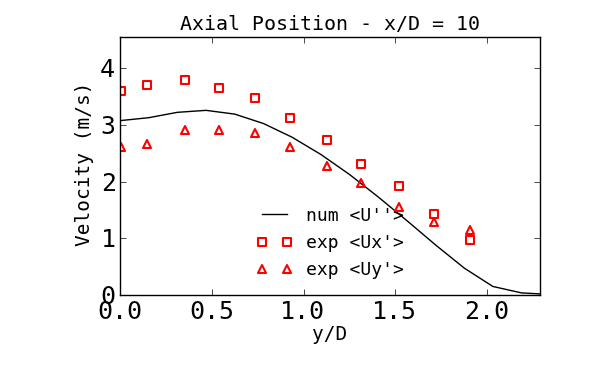
\includegraphics[width=0.5\textwidth]{./figuras/chap5/UU/UUx10.png} \\
(a) & (b) \\
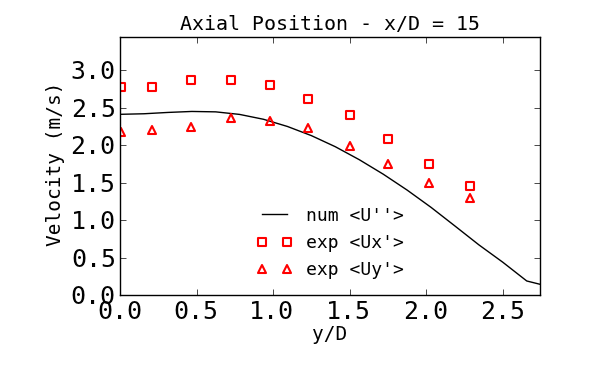
\includegraphics[width=0.5\textwidth]{./figuras/chap5/UU/UUx15.png} & 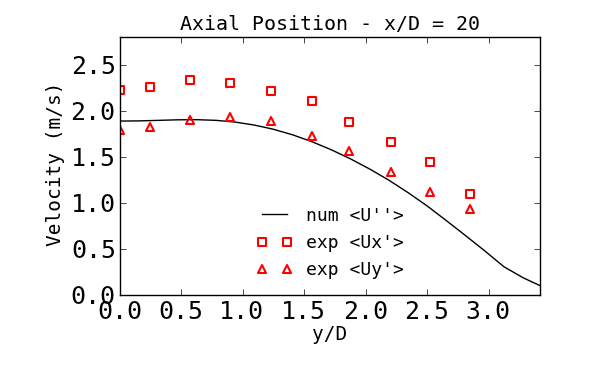
\includegraphics[width=0.5\textwidth]{./figuras/chap5/UU/UUx20.png} \\
(c) & (d) \\
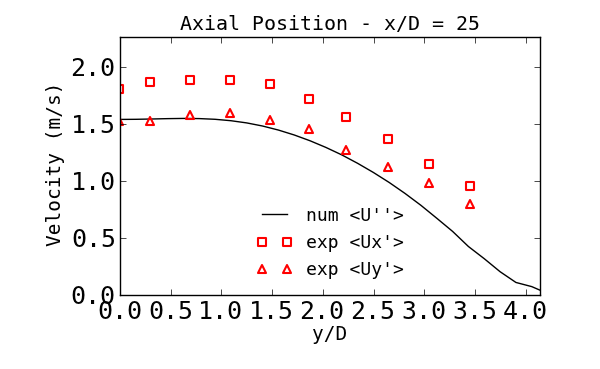
\includegraphics[width=0.5\textwidth]{./figuras/chap5/UU/UUx25.png} &  \\
(e) & \\
\end{tabular}
 \caption{Measured radial profiles of the gas phase velocities $<U''_x>$ and $<U''_y>$ and the characteristic velocity defined for the k-epsilon model $<U''>=\sqrt{2/3 k}$ obtained from the simulation. Each figure shows the profile in a different axial location: $x/D=5$ in (a), $x/D=10$ in (b), $x/D=15$ in (c), $x/D=20$ in (d) and $x/D=25$ in (e). The measurements were obtained from \cite{chen}.}
\label{fig: UUx}
\end{figure}

Returning to the mentioned influence of the discrepancies in the mean axial velocity of the gas phase on the droplet velocities, the lower velocity of the gas increases the droplet slip velocity and causes a larger drag to be felt by them. The obvious conclusion is that the same discrepancy in the gas velocity will be observed in the comparison of experimental and numerical values of the droplet velocities.

Figure \ref{fig: Ux} shows in red squares the radial velocity profile measured  by \cite{chen} for droplets in the class of $10\mu m <D<20\mu m$ in the axial coordinates of: $x/D=5$, $10$, $15$, $20$ and $25$.  For each radial position, the velocity value is the ensemble average of the droplets crossing the laser PDI beams. The droplet velocity obtained in the simulation is also shown as black scattered points representing each of them a different droplet in the computation, no averaging was performed.

It is observed that the computed droplet velocity also becomes systematically lower than the measurements in the downstream direction.

\begin{figure}[!htb]
 \centering
\begin{tabular}{cc}
 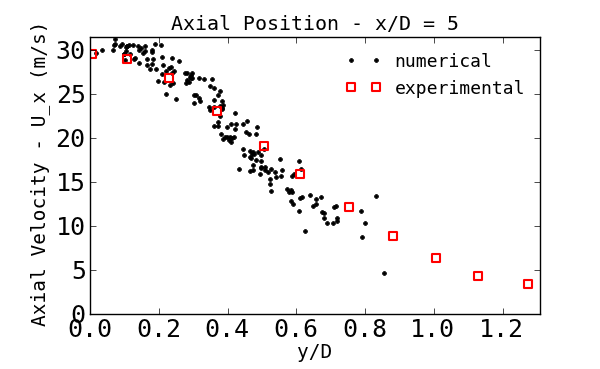
\includegraphics[width=0.5\textwidth]{./figuras/chap5/Ux/Ux_drops/Ux_x5.png} & 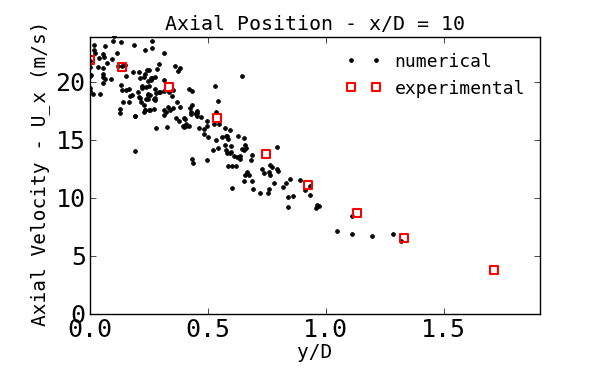
\includegraphics[width=0.5\textwidth]{./figuras/chap5/Ux/Ux_drops/Ux_x10.png} \\
(a) & (b) \\
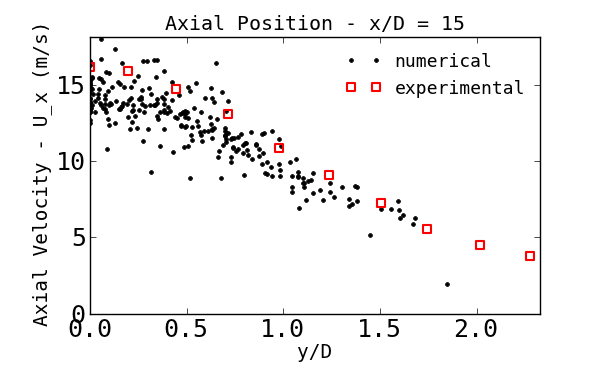
\includegraphics[width=0.5\textwidth]{./figuras/chap5/Ux/Ux_drops/Ux_x15.png} & 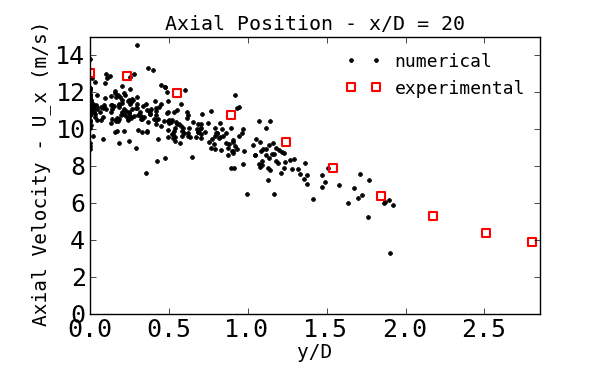
\includegraphics[width=0.5\textwidth]{./figuras/chap5/Ux/Ux_drops/Ux_x20.png} \\
(c) & (d) \\
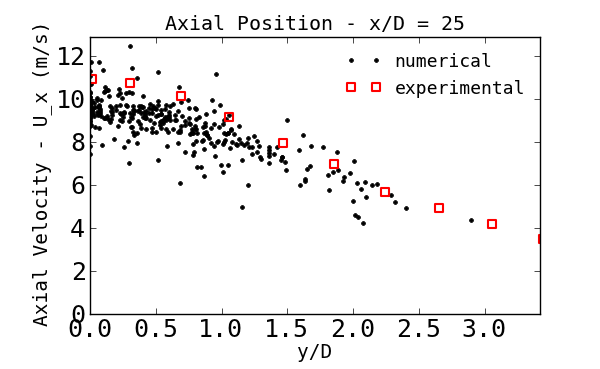
\includegraphics[width=0.5\textwidth]{./figuras/chap5/Ux/Ux_drops/Ux_x25.png} &   \\
(e) & \\
\end{tabular}
 \caption{Red squares present measured radial profiles of mean axial velocity of droplets ($\tilde{U}_{d,x}$) in the size class of $10\mu m <D<20\mu m$. Scattered black dots are the computed velocities for each droplet in the numerical simulation. Each figure shows the velocity profile in the axial coordinate specified above the plot window. The measurements were obtained from \cite{chen}.}
 \label{fig: Ux}
\end{figure}

The last result concerning the droplet velocity is the droplet dispersion: the differences in droplet velocities found in different size classes. Figure \ref{fig: jointUV} shows the numerical instantaneous radial velocity ($U_{y}$) as function of radial coordinate for two extreme size classes: $D< 10\ \mu m$ and $D> 30\ \mu m$. It is seen that the smaller droplets are more sensitive to the gas velocity sampled in the turbulent dispersion model introduced in Chapter \ref{chap: equations}, specially near the nozzle exit. The biggest droplets show a smaller dispersion around the zero mean value because of their higher inertia. As the axial coordinate increases, both behaviors become similar.

\begin{figure}[!htb]
 \centering
\begin{tabular}{cc}
 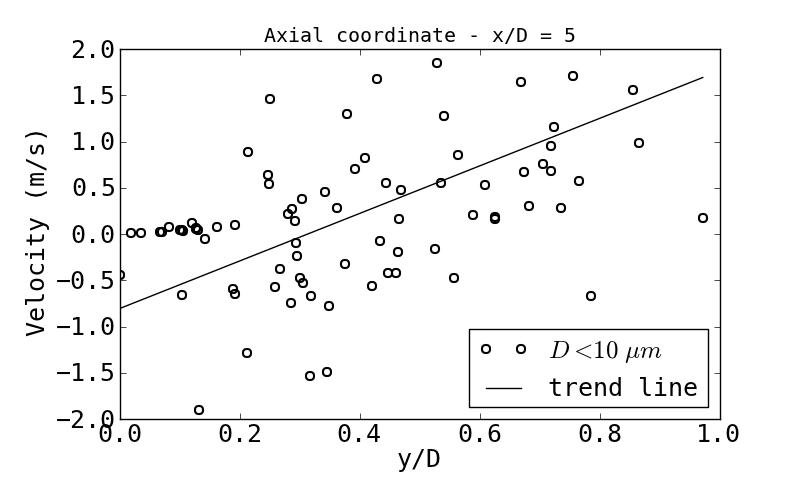
\includegraphics[width=0.5\textwidth]{./figuras/chap5/dispersion/class0_5.png} & 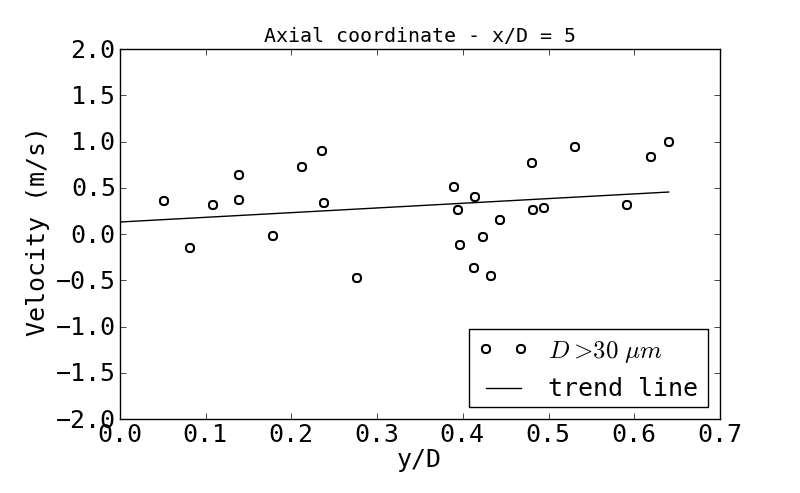
\includegraphics[width=0.5\textwidth]{./figuras/chap5/dispersion/class4_5.png} \\
(a) & (b) \\
 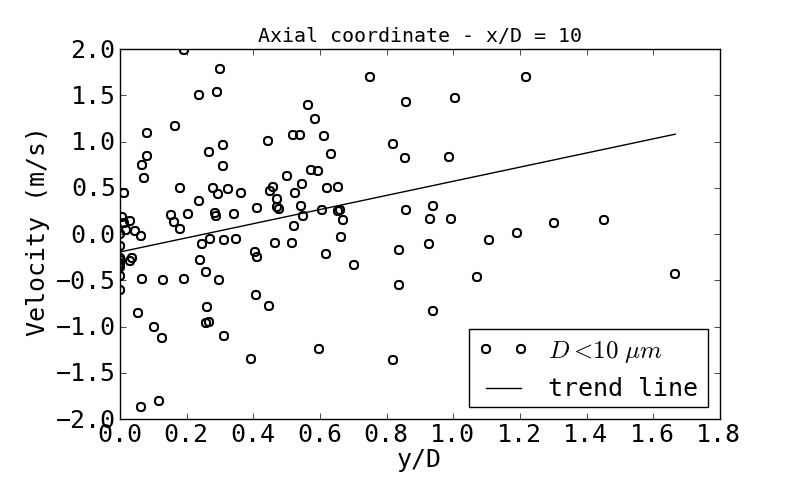
\includegraphics[width=0.5\textwidth]{./figuras/chap5/dispersion/class0_10.png} & 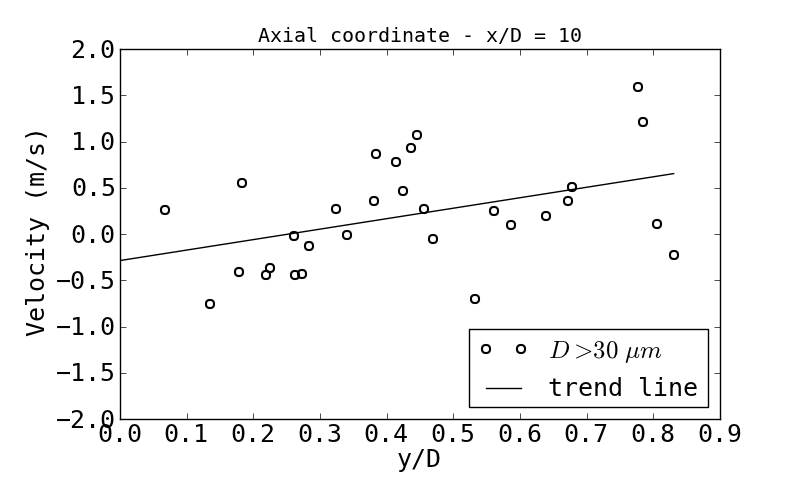
\includegraphics[width=0.5\textwidth]{./figuras/chap5/dispersion/class4_10.png} \\
(c) & (d) \\
 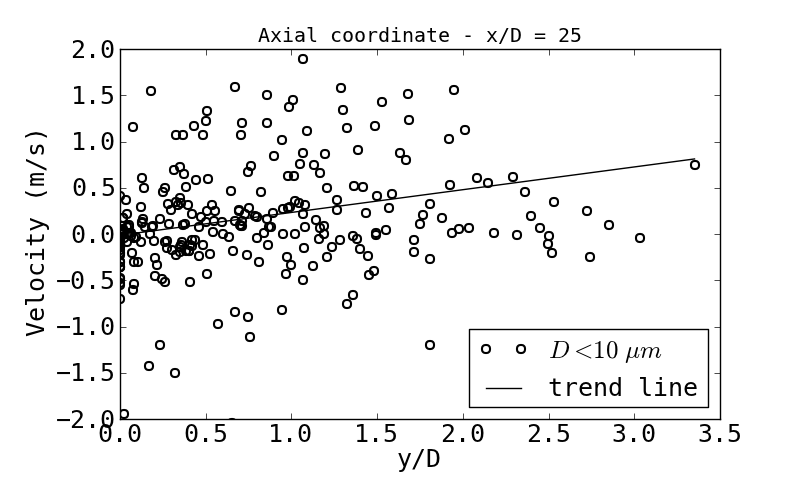
\includegraphics[width=0.5\textwidth]{./figuras/chap5/dispersion/class0_25.png} & 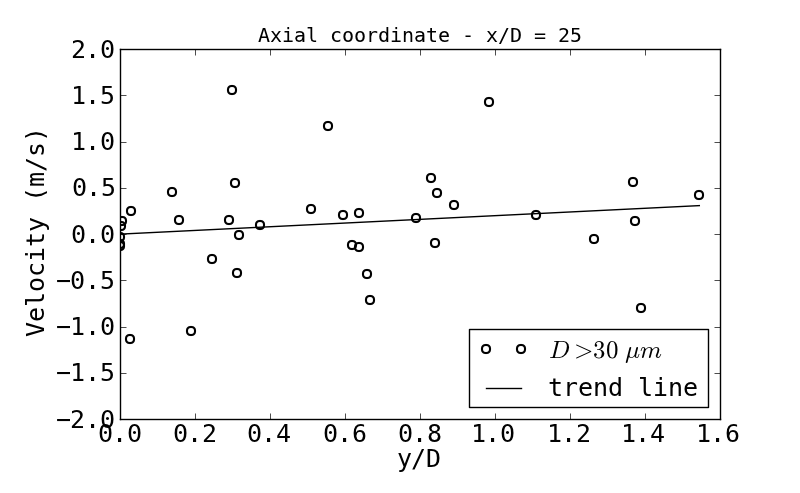
\includegraphics[width=0.5\textwidth]{./figuras/chap5/dispersion/class4_25.png} \\
(e) & (f)
\end{tabular}
 \caption{Scatter plot of the numerical radial velocity of droplets ($U_{y}$) in two different size classes: $D< 10\ \mu m$ on the left or (a), (c) and (e) labels; and $D> 30\ \mu m$ on the right or (b), (d) and (f) labels. The dispersion in the radial velocity is higher for the smaller droplet class and in the vicinity of the nozzle exit.}
\label{fig: jointUV}
\end{figure}

\FloatBarrier
\section{Liquid Mass Flow Rate and Vapor Mass Fluxes}

Correct prediction of droplet evaporation is, together with velocity, of high importance for applications of spray simulation. Reasonably low discrepancies found for droplet velocity in Figure \ref{fig: Ux} already indicates that the evaporation model performed well. This is due to the fact that an incorrect modeling of evaporation would lead to an erroneous droplet diameter, further affecting velocity prediction.

Figure \ref{fig: droplet_flux} shows numerical and experimental liquid mass flow rate for different axial coordinates. Computed values are in good agreement with measurements for $x/D \le 10$. Further downstream, the simulation overpredicts the liquid flow rate. Clearly, this means that droplet evaporation is lower than it should be. In fact, in Figure \ref{fig: vapor_flux}, it is made the comparison of experimental and numerical radial profiles of vapor mass fluxes and the trend is exactly the same: as the axial coordinate increases, less vapor (hence more liquid) is present in simulation than in experiment.

\begin{figure}[!htb]
\centering
  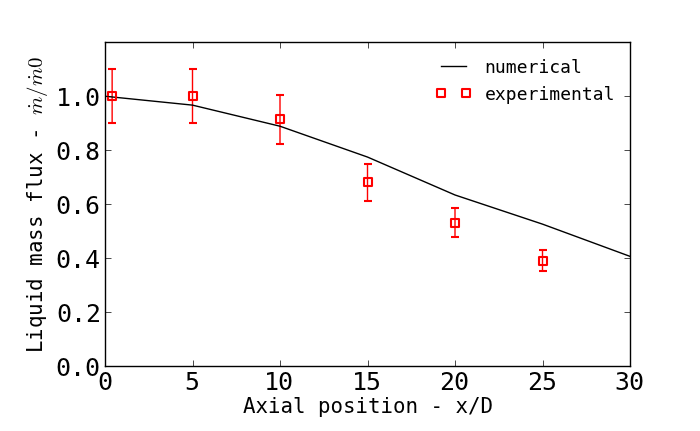
\includegraphics[width=0.6\textwidth]{./figuras/chap5/massflow/drop_mflux.png}
\caption{Droplet mass flow rate at four axial locations. Measurements were obtained from \cite{chen}.}
\label{fig: droplet_flux}
\end{figure} 


\begin{figure}[!htb]
 \centering
\begin{tabular}{cc}
 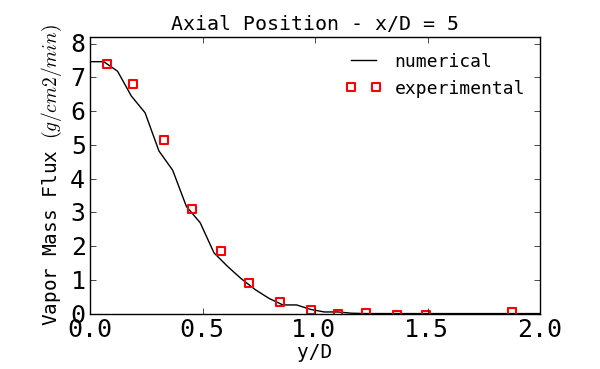
\includegraphics[width=0.45\textwidth]{./figuras/chap5/massflow/mvapor5.png} & 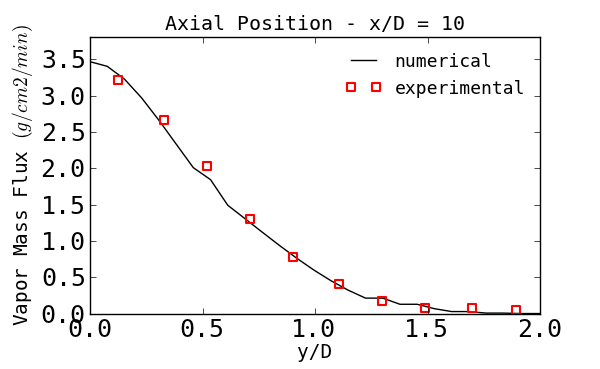
\includegraphics[width=0.45\textwidth]{./figuras/chap5/massflow/mvapor10.png} \\
(a) & (b) \\
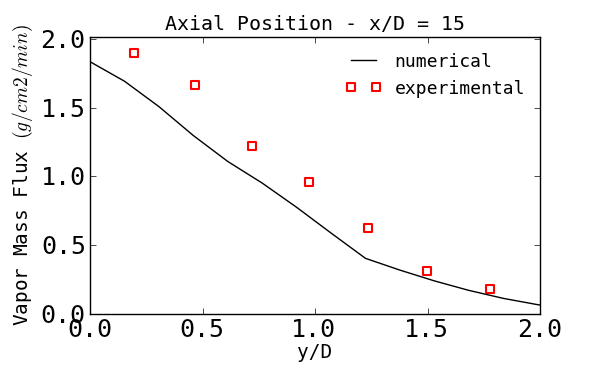
\includegraphics[width=0.45\textwidth]{./figuras/chap5/massflow/mvapor15.png} & 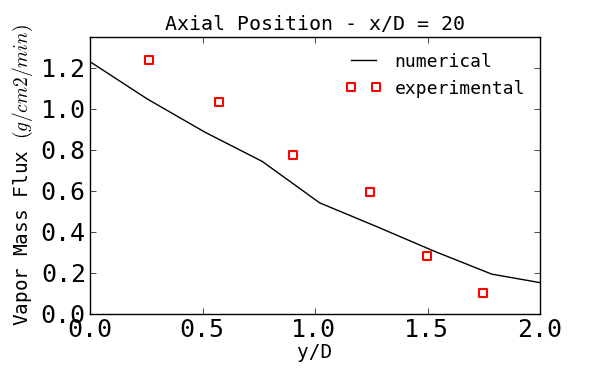
\includegraphics[width=0.45\textwidth]{./figuras/chap5/massflow/mvapor20.png} \\
(c) & (d)
\end{tabular}
 \caption{Radial profiles of mean axial mass flux of acetone vapor: $\dot{m}''_{ac}=\rho \bar{Y}_{ac} \tilde{U}_x$. The measurements were obtained from \cite{chen}.}
 \label{fig: vapor_flux}
\end{figure}

The underestimation of evaporation rate has also been noticed in a large-eddy simulation performed by \cite{bini}, where it was discussed the effect of a subgrid model to the evaporation. It is said that the lack of a subgrid model affects evaporation mainly in the jet core, where the mean vapor mass fraction might be saturated, but negative oscillations might allow for extra vaporization. In fact, the evaporation model presented in Chapter \ref{chap: equations} only deals with the averaged flow properties, and the temperature and mass fraction oscillations, ($T''$) and ($Y''_{ac}$), are not taken into account.

Surely, for a large-eddy simulation, the lack of a subgrid model is less severe than in RANS modeling since at least the non-filtered oscillations are present. 

A stochastic model for RANS simulation was proposed in \cite{santanu}. The proposed approach was to establish stochastic behaviors for $T''$ and $Y''_{ac}$ and use the instantaneous values of them ($T$ and $Y_{ac}$) in the heating and evaporation models. The results, however, did not improve significantly in the case it studied. This approach implies an odd assumption that the experimental correlations used for the droplet models, which were developed for a non-oscillating gas field, would work for an oscillating situation by only using instantaneous flow properties. A more profound discussion is found in \cite{sirignano}, where directly modeling of the Sherwood and the Nusselt numbers is suggested. This is the same approach used in \cite{bini} with good results.

It must also be pointed that uncertainties in the gas mean velocity also affect the droplet heating and evaporation prediction again because of the different slip velocity. The correct attempt to improve accuracy of the present computation would be to adjust the turbulence model to firstly correct the gas mean velocity and see the new evaporation rates. Next, a stochastic subgrid model for the heat and mass transfer coefficients could be studied.

\begin{figure}[!htb]
 \centering
\begin{tabular}{c}
 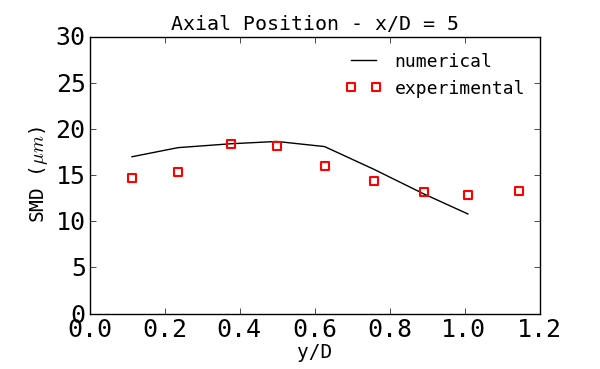
\includegraphics[width=0.5\textwidth]{./figuras/chap5/smd/smd5.png} \\
(a) \\
 \includegraphics[width=0.5\textwidth]{./figuras/chap5/smd/smd15.png} \\
(b) \\
 \includegraphics[width=0.5\textwidth]{./figuras/chap5/smd/smd25.png} \\
(c) 
\end{tabular}
 \caption{Numerical and experimental radial profiles of Sauter mean diameter (SMD). The measurements were obtained from \cite{chen}.}
 \label{fig: SMDprofile}
\end{figure}

The last studied property of the spray is the droplet Sauter mean diameter (SMD). Figure \ref{fig: SMDprofile} shows the numerical and experimental radial profiles of SMD.

The computed Sauter mean diameter shows a good agreement with measurements, in despite of the uncertainty about the droplet size distribution in the boundary conditions and the higher liquid flow rates in Figure \ref{fig: droplet_flux}. This may also be a consequence of the low variance in droplet diameter in the nozzle injection.

This agreement also confirms that the velocity discrepancy is caused by the anomalous jet spread rate. As discussed previously, if diameters were also in disagreement, the predicted drag force on the droplets would be further incorrect.


\FloatBarrier


\chapter{Conclusions}\label{chap: conclusion}
%\section{Considera��es finais}

This work presented a set of equations to model the evolution of a spray jet and its numerical solution. Computations were compared to available measurements indicating a good general prediction of flow quantities with some disagreements susceptible to improvements in the droplet velocity and evaporation rate.

Velocity of both gas and liquid phases were underpredicted due to the high turbulent viscosity computed by the turbulence model. It is suggested in the literature that the discrepancies for a round jet may be diminished by changing the model coefficients and reducing the turbulent length scale in jet inlet boundary conditions.

Evaporation rate was underpredicted after the jet developing region. Turbulence effects on Nusselt and Sherwood numbers were not modeled and this is believed to decrease evaporation, specially in the jet core, as reported by \cite{bini}.

Further, disagreements in the prediction of gas velocity may also have contributed to differences in the evaporation rate. The maximum error in liquid mass flow rate at some axial location was about $20\%$.

The shape of radial profile of vapor mass fluxes was well predicted. The same can be said to the SMD radial profiles.

Future work could explore improvements in the round jet turbulence modeling and new heating and evaporation models for RANS simulations accounting for fluctuations of flow properties. Something similar to what was done in \cite{bini} could serve as a starting point.

The hypothesis of unity Prandtl and Schmidt numbers was also not tested.

Finally, the OpenFOAM source code offers powerful and flexible libraries that may be adapted to user needs. It consists of a great platform for collaborative code development in fluid dynamics. It is also an alternative for industry in the development of in-house solutions. 



% Referencias Bibliograficas
\begin{spacing}{1.0}
\begin{flushleft}
%   \nocite{*}
\bibliography{references}
\end{flushleft}
\end{spacing}


% Apendices
\appendix
\chapter{Appendix}
\section{Sensible Enthalpy Equation}\label{appendix 1}

The aim of this section is to start from the total energy equation for a compressible flow of a perfect gas mixture and arrive to the sensible enthalpy equation, clarifying the confusion that might be caused by the different forms of energy (or enthalpy) equations. 

For a mixture of $M$ perfect gases, the total energy is defined as the sum of the chemical, kinetic, potential and sensible energies:
\begin{equation}
\begin{split}
 e_t &= \underbrace{\int_{T_0}^T C_v dT -RT_0/W}_{\text{sensible}} + \underbrace{\sum_{k=1}^{M} \Delta h_{f,k}^{0} Y_k}_{\text{chemical}} + \underbrace{\frac{1}{2}\left( \bv{U}\cdot \bv{U} \right)}_{\text{kinetic}} - \underbrace{\int_{\gamma} \bv{g} \cdot \bv{ds}}_{\text{potential}}
\\ &= \sum_{k=1}^{M} e_{t,k} Y_k \, ,
\end{split}
\end{equation}
where $\Delta h_{f,k}^{0}$ is the mass enthalpy of formation of species $k$ at a reference temperature $T_0$. $\gamma$ is a path, with respect to some reference position, in the volumetric force field $\bv{g}$.

The sensible energy $(e_s)$ is solely the parcel sensitive to temperature variations. The thermal energy $(e)$ comprises both the chemical and sensible energies (the total energy subtracted of the mechanical energy). 

The conservation equation for the total energy, see \cite{poinsot2005theoretical}, reads:
\begin{equation}\label{ap: et}
 \frac{\partial \rho e_t}{\partial t} + \nabla \cdot \left( \rho \bv{U} e_t\right) = \nabla \cdot \bv{J} + \nabla \cdot \left( \bv{\sigma} \cdot \bv{U} \right) + \Phi + \rho \sum_{k=1}^N Y_k \bv{g}_k \cdot \left( \bv{U}+\bv{V_k}\right) \, ,
\end{equation}
where $\bv{g}_k$ is the volumetric force on species $k$, $\Phi$ is the heat source term, $\bv{\sigma}$ is the stress tensor $\bv{\sigma} = \bv{\tau} -p\bv{I}$ and
\begin{equation}
 \bv{J} =  \kappa \nabla T - \rho \sum_{k=1}^{M} h_{k} \bv{V}_k Y_k \, .
\end{equation}

The heat source term is due to external heat added to the system, e.g. an electric spark or a radiative flux. It must not be confounded with the heat released by combustion (or a chemical reaction), which is already contained in the system in the form of chemical energy. The  heat released in combustion is obtained by computing the difference in the enthalpy of formation of reactants and products.

The following manipulations of \eqref{ap: et} consist in substituting total energy with total enthalpy, subtracting the mechanical energy and then subtracting the chemical enthalpy. The resulting equation is that of the sensible enthalpy.

The relation between total energy $(e_t)$ and total enthalpy $(h_t)$ is $e_t=h_t - p/\rho$. The total derivative of $e_t$ in terms of $h_t$ then becomes:
\begin{equation}
  \frac{\partial \rho e_t}{\partial t} + \nabla \cdot \left( \rho \bv{U} e_t\right) =\frac{\partial \rho h_t}{\partial t} + \nabla \cdot \left( \rho \bv{U} h_t\right) + \frac{\partial p}{\partial t} + \nabla \cdot \left( p \bv{U}\right) \, .
\end{equation}

Substituting in \eqref{ap: et},

\begin{equation}\label{ap: ht}
\begin{split}
 \frac{\partial \rho h_t}{\partial t} + \nabla \cdot \left( \rho \bv{U} h_t\right) &= \frac{\partial p}{\partial t} + \nabla \cdot \bv{J} + \nabla \cdot \left[ \left( \bv{\sigma} + p\bv{I} \right) \cdot \bv{U} \right] + \Phi + \rho \sum_{k=1}^N Y_k \bv{g}_k \cdot \left( \bv{U}+\bv{V_k}\right)  \\
& = \frac{\partial p}{\partial t} + \nabla \cdot \bv{J} + \nabla \cdot \left( \bv{\tau}\cdot \bv{U} \right) + \Phi + \rho \sum_{k=1}^N Y_k \bv{g}_k \cdot \left( \bv{U}+\bv{V_k}\right)
\, .
\end{split}
\end{equation}

The conservation equation of kinetic energy, here denoted by $\Pi = 1/2 \left( \bv{U} \cdot \bv{U}\right)$, is obtained by the scalar product of the momentum equation and $\bv{U}$:
\begin{equation}\label{ap: kinetic}
 \frac{\partial \rho \Pi}{\partial t} + \nabla \cdot \left( \rho \bv{U} \Pi\right) = \bv{U} \cdot \left( \nabla \cdot \sigma \right) +\rho \sum_{k=1}^{M} Y_k \left( \bv{g}_k \cdot \bv{U} \right)  \, .
\end{equation}

Subtracting Equation \eqref{ap: kinetic} from \eqref{ap: ht}, the thermal enthalpy equation is obtained:
\begin{equation}\label{ap: h}
 \frac{\partial \rho h}{\partial t} + \nabla \cdot \left( \rho \bv{U} h\right) = \frac{\partial p}{\partial t} + \nabla \cdot \bv{J} +  \left[ \nabla \cdot \left( \tau \cdot \bv{U} \right) - \bv{U} \cdot \left( \nabla \cdot \sigma \right)  \right] + \Phi \, ,
\end{equation}

using the definition of $\sigma$ and after some algebra shown below
\begin{equation}
\begin{split}
 \nabla \cdot \left( \tau \cdot \bv{U} \right) - \bv{U} \cdot \left( \nabla \cdot \sigma \right) &= \left[ \tau : \nabla \bv{U} + \left( \nabla \cdot \tau \right) \cdot  \bv{U} \right] - \left[ \left( \nabla \cdot \bv{\tau} \right) - \nabla p \right] \cdot \bv{U} \\
&= \bv{\tau}:\nabla \bv{U}+ \bv{U} \cdot \nabla p \, ,
\end{split} 
\end{equation}

the conservation equation for the thermal enthalpy becomes:
\begin{equation}\label{ap: enthalpy}
  \frac{\partial \rho h}{\partial t} +  \nabla \cdot \left( \rho h \bv{U} \right) = \frac{Dp}{Dt} + \nabla \cdot \bv{J} +  \bv{\tau} : \nabla\bv{U} + \Phi\, .
\end{equation}

The relation between thermal and sensible enthalpy is
\begin{equation}
 h = h_s+\sum_{k=1}^{M} \Delta h^{0}_{f,k} Y_k \,.
\end{equation}

Subtituing into $\bv{J}$ and then in \eqref{ap: enthalpy}:
\begin{equation}
\begin{split}
 \bv{J} &=  \underbrace{\kappa \nabla T - \rho \sum_{k=1}^{M} h_{s,k} \bv{V}_k Y_k}_{\bv{J}_s} - \rho \sum_{k=1}^{M} \Delta h^{0}_{f,k} \bv{V}_k Y_k \\
& = \bv{J}_s - \rho \sum_{k=1}^{M} \Delta h^{0}_{f,k} \bv{V}_k Y_k \, .
\end{split}
\end{equation}

\begin{equation}
\begin{split}
\frac{\partial \rho h_s}{\partial t} +  \nabla \cdot \left( \rho h_s \bv{U} \right) &=\\
 &-  \sum_{k=1}^{M} \Delta h^{0}_{f,k} \left[ \frac{\partial \rho Y_k }{\partial t} + \nabla \cdot \left( \rho \left( \bv{U} + \bv{V}_{k}\right) Y_k \right)  \right]  \\
  &+\frac{Dp}{Dt} + \nabla \cdot \bv{J}_s +  \bv{\tau} : \nabla\bv{U} + \Phi\, .
\end{split}
\end{equation}

Using the species conservation equation to substitute the terms inside the brackets, the final form of sensible enthalpy equation is obtained:
\begin{equation}
\begin{split}
\frac{\partial \rho h_s}{\partial t} +  \nabla \cdot \left( \rho h_s \bv{U} \right) &= \omega_H+\frac{Dp}{Dt} + \nabla \cdot \bv{J}_s +  \bv{\tau} : \nabla\bv{U} + \Phi 
\end{split}
\end{equation}
where $\omega_H$ is the heat released in combustion (or some chemical reaction):
\begin{equation}
 \omega_H = - \sum_{k=1}^{M} \Delta h^{0}_{f,k}  S_{Yk} \, .
\end{equation}

\section{Extra Figures}\label{appendix 2}
\begin{figure}[h]
 \centering
 \includegraphics[height=0.7\textheight]{./figuras/appA2/visit_Td.png}
 % k_bc.png: 800x493 pixel, 100dpi, 20.32x12.52 cm, bb=
 \caption{Temperature of droplets. The computational domain is only half of the shown above, it is here mirrored for visualization purpose.}
 \label{fig: dropT}
\end{figure}

\clearpage
\begin{figure}
 \centering
 \includegraphics[height=0.9\textheight]{./figuras/appA2/visit_U.png}
 \caption{Magnitude of droplet velocities. The computational domain is only half of the shown above, it is here mirrored for visualization purpose.}
 \label{fig: dropU}
\end{figure}

\clearpage
\begin{figure}
\begin{center}
  \includegraphics[height=0.9\textheight]{./figuras/appA2/visit_T.png}
 \end{center}
 \caption{Gas mean temperature field $\tilde{T}$. The computational domain is only half of the shown above, it is here mirrored for visualization purpose.}
 \label{fig: field_T}
\end{figure}

\clearpage
\begin{figure}
\begin{center}
  \includegraphics[height=0.9\textheight]{./figuras/appA2/visit_Ux.png}
 \end{center}
\caption{Gas mean velocity magnitude $|\tilde{\bv{U}}|$. The computational domain is only half of the shown above, it is here mirrored for visualization purpose.}
 \label{fig: field_U}
\end{figure}

\clearpage
\begin{figure}
\begin{center}
  \includegraphics[height=0.9\textheight]{./figuras/appA2/visit_k.png}
 \end{center}
 \caption{Gas mean turbulent kinetic energy. The computational domain is only half of the shown above, it is here mirrored for visualization purpose.}
 \label{fig: field_k}
\end{figure}

\clearpage
\begin{figure}
\begin{center}
  \includegraphics[height=0.9\textheight]{./figuras/appA2/visit_aC3H6O.png}
 \end{center}
 \caption{Mean of acetone vapor mass concentration - $\tilde{Y}_{ac}$. The computational domain is only half of the shown above, it is here mirrored for visualization purpose.}
 \label{fig: aa}
\end{figure}

\FloatBarrier


\section{Equation Discretization and PISO Algorithm}\label{appendix 3}

\begin{figure}[h]
 \centering
\begin{tabular}{cc}
 \includegraphics[width=0.55\textwidth]{./figuras/appA3/finite_volume.png}
\end{tabular}
 \caption{Finite volume discretization, reproduced from \cite{foamDev}.}
 \label{fig: fvm}
\end{figure}

A brief explanation of PISO algorithm and equation discretization as used in this work is here presented. The notation of equations follow OpenFOAM formulation explained in \cite{jasak}.

Superscripts \textbf{o} and \textbf{n} denote values from previous and current time-steps, respectively. \textbf{*} and \textbf{**} subscripts are used to denote intermediate fields computed before the final value of the time-step.

Subscripts \textbf{P} and \textbf{N} denote values stored in the center of owner and neighbor cells.  See Figure \ref{fig: fvm} for the geometric representation of two neighboring cells.

Subscript \textbf{f} indicates values interpolated from cell center to a face center. Advective terms were interpolated using the simple upwind scheme. The linear scheme was used for remaining interpolations. Setup of \verb|fvSchemes| input file is presented after PISO algorithm.

\clearpage
\textbf{Beginning of a new time-step:}
\begin{itemize}
  \item Evolve spray: move droplets and compute new spray source terms using old gas properties.

  \item Solve continuity equation for first density estimate $\bar{\rho}^{*}$:
    \begin{equation}
      \frac{\bar{\rho}^{*}-\bar{\rho}^{o}}{\Delta t} V_P +\sum_f F^{o} = S_m V_P \, ,
    \end{equation}
    where $F^{o}$ is the mass flow through cell faces from previous time-step:
  \begin{equation}
    F^{o}=\left(\bar{\rho}^{o}\tilde{\bv{U}}^{o}\right)_f\cdot \bv{S}_f \, .
  \end{equation} 
  This equation provides an explicit formulation for $\bar{\rho}^{*}$.

  \item Solve momentum equation for first velocity estimate $\bv{U}^{*}$ (momentum predictor):
    \begin{equation}
      \frac{\bar{\rho}^{*}\tilde{\bv{U}}^{*}-\bar{\rho}^{o}\tilde{\bv{U}}^{o}}{\Delta t} V_P + \sum_f F^{o}\tilde{\bv{U}}_f^{*} = \sum_f \bv{\tilde{\tau}}_f \cdot \bv{S}_f+\left(\bar{\rho}^{*}\bv{g}+\bv{S}_{mom} \right)V_P - \sum_f \bar{p}_{2,f}^{o}\bv{S}_{f}
    \end{equation}
    where 
    \begin{equation}
    \tilde{\bv{\tau}}=\underbrace{\sum_f \left( \mu_{eff}\nabla\tilde{\bv{U}}^{*} \right)_f \cdot \bv{S}_f}_{\text{implicit}} - \underbrace{\sum_f \mu_{eff,f}\left[\nabla \bv{\tilde{U}}^{o,T} -\frac{2}{3}\left(\nabla\cdot\tilde{\bv{U}}^{o}\right)\bv{I}\right]_f \cdot \bv{S}_f}_{\text{explicit}}
    \end{equation}
    The equation may be rewritten in a reduced semi-discretized form as:
    \begin{equation}
      \tilde{\bv{U}}_P^{*} = \frac{1}{a_P}\bv{H}(\tilde{\bv{U}}^{o})-\frac{1}{a_P}\nabla \bar{p}_2 \, .
    \end{equation}
    
  \item Solve species equation for $\tilde{Y}^{n}_k$:
  \begin{equation}
    \frac{\bar{\rho}^{*}\tilde{Y}_k^{n}-\bar{\rho}^{o}\tilde{Y}_k^o}{\Delta t} V_P +\sum_f F^{o}\tilde{Y}_{k,f}^{n} = \sum_f \left(\mu_{eff}\nabla\tilde{Y}_{k}^{n}\right)_f \cdot \bv{S}_f + S_{Yk} V_P
  \end{equation}

  \item Solve enthalpy equation for $\tilde{h}_{s}^{n}$:
  \begin{equation}
    \frac{\bar{\rho}^{*}\tilde{h}_s^{n}-\bar{\rho}^{o}\tilde{h}_s^o}{\Delta t} V_P +\sum_f F^{o}\tilde{h}_{s,f}^{n} = \sum_f \left(\mu_{eff}\nabla\tilde{h}_{s}^{n}\right)_f \cdot \bv{S}_{f}  + S_{hs} V_P
  \end{equation}
\end{itemize}

The computation of new pressure ($\bar{p}^n$) and velocity ($\bv{\tilde{U}}^n$) fields is performed in a iterative manner shown in next page.

\begin{tabular}{|p{0.95\textwidth}|} \hline
\textbf{PISO Loop (pressure-velocity coupling)} \\
\hline
Update $\rho$ with state equation using new temperature: $\bar{\rho}^{**} = p_0 \tilde{W} / R \tilde{T}^{n}$ \, ;\\
Compute second estimate of velocity ($\bv{U}^{**}$) without pressure contribution:
\begin{equation}
\tilde{\bv{U}}_P^{**} = \frac{1}{a_P}\bv{H}(\tilde{\bv{U}}^{*}) \, ;
\end{equation}

Update mass flow through cell faces using new density and velocity:
\begin{equation}
F^{*}=\left(\bar{\rho}^{**}\tilde{\bv{U}}^{**}\right)_f\cdot \bv{S}_f \, ;
\end{equation}

Solve pressure equation for the new dynamic pressure field $\bar{p}_2^n$:
\begin{equation}
  \sum_f \left[ F^{*} - \bv{S}_f\cdot\left(\frac{\bar{\rho}^{**}}{a_P}\nabla \bar{p}_2^{n} \right)_f \right] = S_m V_P \, ;
\end{equation}

Solve continuity equation for new density ($\bar{\rho}^n$) with $F^{*}$:
\begin{equation}
\frac{\bar{\rho}^{n}-\bar{\rho}^{o}}{\Delta t} V_P +\sum_f F^{*} = S_m V_P \, ;
\end{equation}

Compute the new velocity ($\tilde{\bv{U}}^{n}$) adding pressure contribution (momentum-corrector) and update mass fluxes:
\begin{equation}
\tilde{\bv{U}}^{n} = \tilde{\bv{U}}^{**} - \frac{1}{a_P}\sum_f \bar{p}_{2,f}^{n}\bv{S}_f \, ,
\end{equation}
\begin{equation}
 F^{n}=\left(\bar{\rho}^{n}\tilde{\bv{U}}^{n}\right)_f\cdot \bv{S}_f \, .
\end{equation}\\
\hline
\end{tabular}
PISO loop may be repeated inside the same time-step by setting $\tilde{\bv{U}}^{n}=\tilde{\bv{U}}^{o}$ and performing all steps again.

\clearpage
\begin{singlespace}
Setup of discretization schemes in \verb|fvSchemes| input file:
\begin{verbatim}
/*--------------------------------*- C++ -*----------------------------------*\
| =========                 |                                                 |
| \\      /  F ield         | OpenFOAM: The Open Source CFD Toolbox           |
|  \\    /   O peration     | Version:  1.7.1                                 |
|   \\  /    A nd           | Web:      www.OpenFOAM.com                      |
|    \\/     M anipulation  |                                                 |
\*---------------------------------------------------------------------------*/
FoamFile
{
    version     2.0;
    format      binary;
    class       dictionary;
    location    "system";
    object      fvSchemes;
}
// * * * * * * * * * * * * * * * * * * * * * * * * * * * * * * * * * * * * * //

ddtSchemes
{
    default         Euler;
}

gradSchemes
{
    default         none;

    //pEqn.H, velocity correction in PISO.
    grad(pd)         Gauss linear;
    
    // strain tensor
    grad(U)			Gauss linear;
}

divSchemes
{
    default         none;
    div(phi,rho)    Gauss upwind;
    div(phi,U)      Gauss upwind;
    div(phi,k)      Gauss upwind;
    div(phi,epsilon) Gauss upwind;
    div(phi,Yi_h)   Gauss upwind; // divergent scheme for Yk and hs
    div((muEff*dev2(grad(U).T()))) Gauss linear;
}

laplacianSchemes
{
    default         none;
    
    //UEq.H
    laplacian(muEff,U) Gauss linear uncorrected;
    
    //YEq.H
    laplacian(muEff,aC3H6O) Gauss linear uncorrected;
    laplacian(muEff,N2) Gauss linear uncorrected;
    laplacian(muEff,O2) Gauss linear uncorrected;
    laplacian(muEff,CO2) Gauss linear uncorrected;
    laplacian(muEff,H2O) Gauss linear uncorrected;
    
    //hsEq.H
    laplacian(alphaEff,hs) Gauss linear uncorrected;
    
    //pEq.H
    laplacian((rho*(1|A(U))),pd) Gauss linear uncorrected;
    
    //epsEq <kEpsilon.C>
    laplacian(DepsilonEff,epsilon) Gauss linear uncorrected;
    
    //kEq <kEpsilon.C>
    laplacian(DkEff,k) Gauss linear uncorrected;
}

interpolationSchemes
{
    default         linear;
    interpolate(HbyA) linear;
}

snGradSchemes
{
    default         uncorrected;
}

fluxRequired
{
    default         no;
    pd;
}
// * * * * * * * * * * * * * * * * * * * * * * * * * * * * * * * * * * * * * //
\end{verbatim}
\end{singlespace}

% Anexos
%\annex
%\chapter{Annex}
% Glossario
\itaglossary
\printglossary

% Folha de Registro do Documento
% Valores dos campos do formulario
\FRDitadata{25 de novembro de 2011}
\FRDitadocnro{DCTA/ITA/DM-054/2011}
%\FRDitaorgaointerno{Instituto Tecnol\'{o}gico de Aeron\'{a}utica - ITA}
\FRDitapalavrasautor{Spray; Escoamento multif\'{a}sico; Combust\~{a}o; M\'{e}todo de volumes finitos; OpenFOAM.}
\FRDitapalavrasresult{Pulverizadores; Escoamento multif\'{a}sico; Combust\~{a}o; M\'{e}todo de volumes finitos; An\'{a}lise num\'{e}rica; Simula\c{c}\~{a}o do escoamento; F\'{i}sica.}
\FRDitaresumo{
This work consists in a numerical simulation of a spray jet: a two-phase flow composed by a gaseous and a liquid phase. The gaseous phase is treated as a continuous medium, and the liquid phase is treated as a dispersed phase. An asymptotic approximation of zero Mach number was applied to the gaseous phase in order to account for density variations due to temperature gradients without dealing with extra complexities of the fully compressible flow formulation. The effects of turbulence on the gas flow were modeled using the concept of turbulent viscosity determined by a system of two partial differential equations, the so called k-epsilon model. The liquid dispersed phase was modeled as point-particles, to whom thermodynamic properties and 0-d models for momentum, heat and mass transfers were assigned. The gaseous phase was discretized and numerically solved using the finite volume method. The numerical results were compared to measurements and a reasonable prediction was found. It was verified, though, underestimations of droplet velocity and evaporation rate.
}
\FRDitaapresentacao{ITA, S\~{a}o Jos\'{e} dos Campos. Curso de Mestrado. Programa de P\'{o}s-Gradua\c{c}\~{a}o em Engenharia Aeron\'{a}utica e Mec\^{a}nica. \'{A}rea de Aerodin\^{a}mica, Propuls\~{a}o e Energia. Orientador: Prof. Marcelo Jos\'{e} Santos de Lemos. Defesa em 25/11/2011. Publicada em 2011.}
%  Primeiro Parametro: Nacional ou Internacional -- N/I
%  Segundo parametro: Ostensivo, Reservado, Confidencial ou Secreto -- O/R/C/S
\FRDitaOpcoes{N}{O}
% Cria o formulario
\itaFRD

\end{document}
% Fim do Documento.
% 
